\appendix
\chapter{Galapagos Instruction Set Architecture Documentation} \label{appendix:isa}
\newpage
\includepdf[pages=-]{isa/isa.pdf}

\chapter{PCB schematics} \label{appendix:pcb-schematics}
\newpage
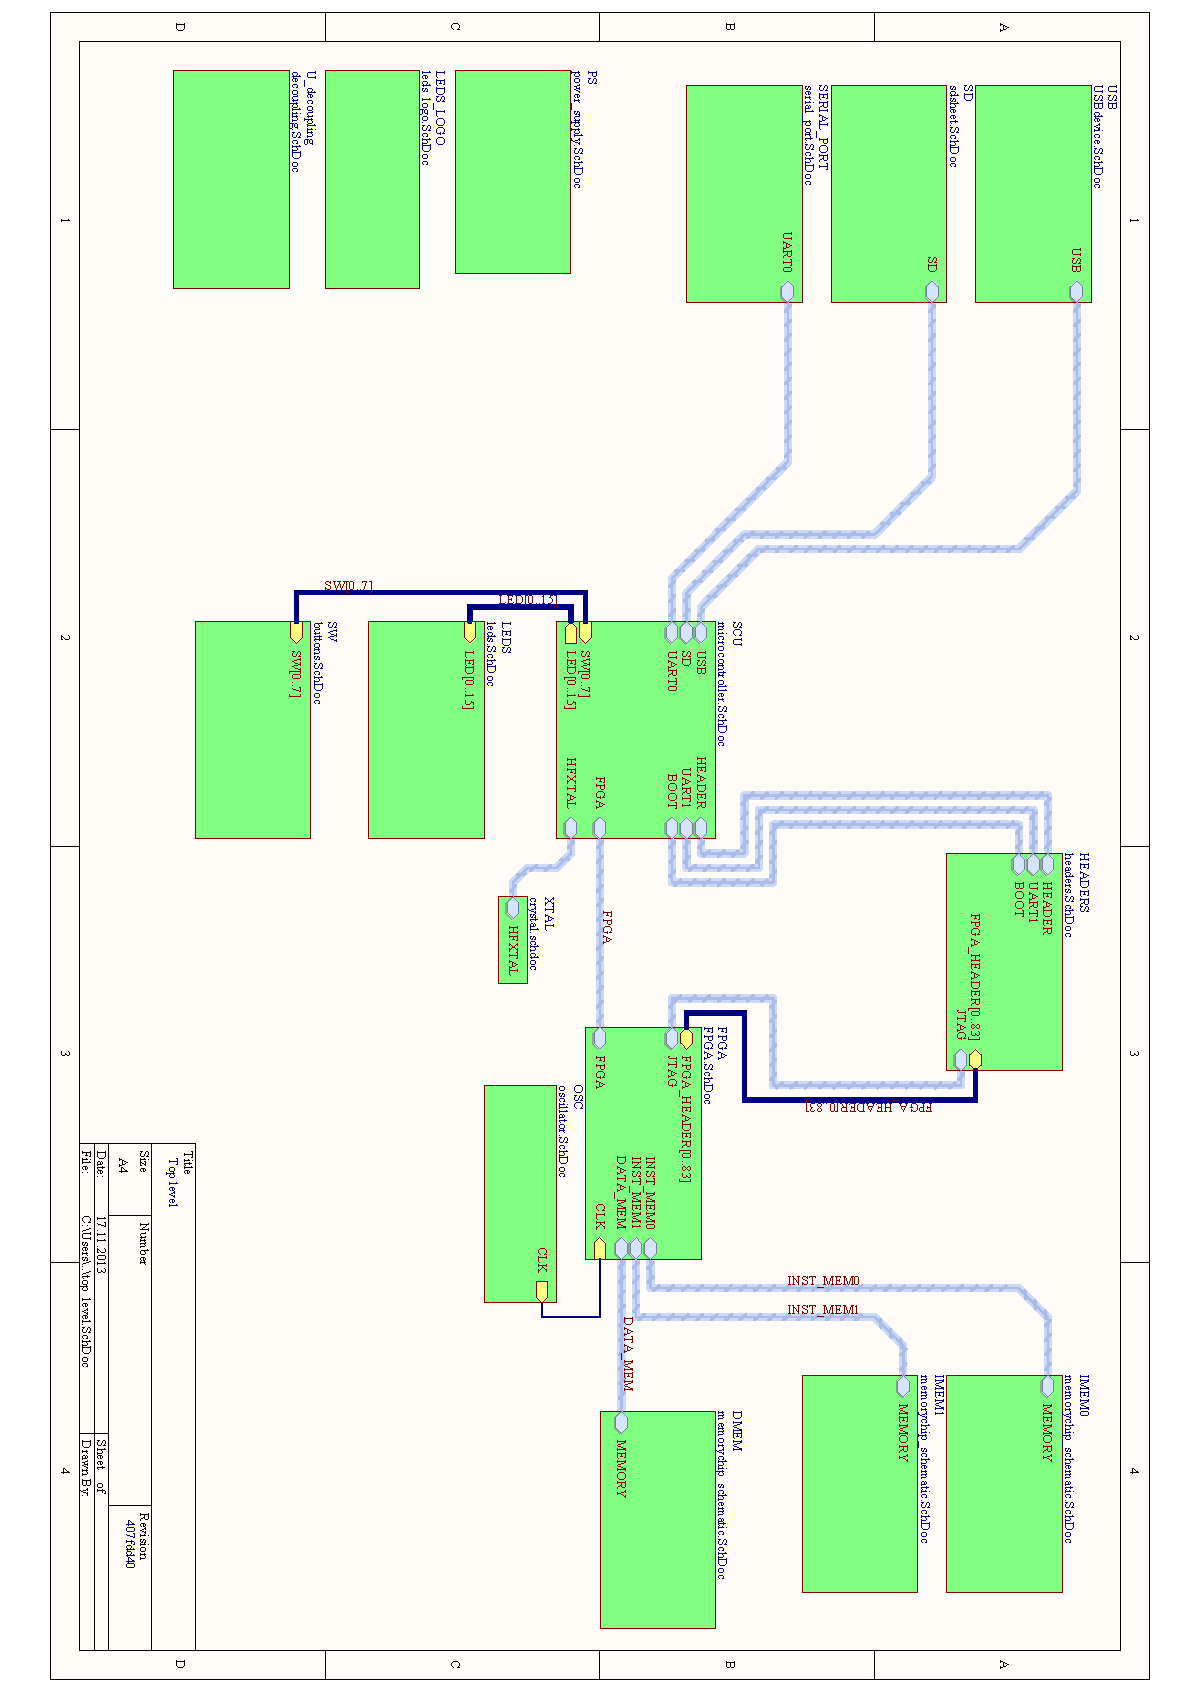
\includepdf[pages=-]{appendix/PCB_TDT4295_NTNU_2013_rotated.16.pdf}
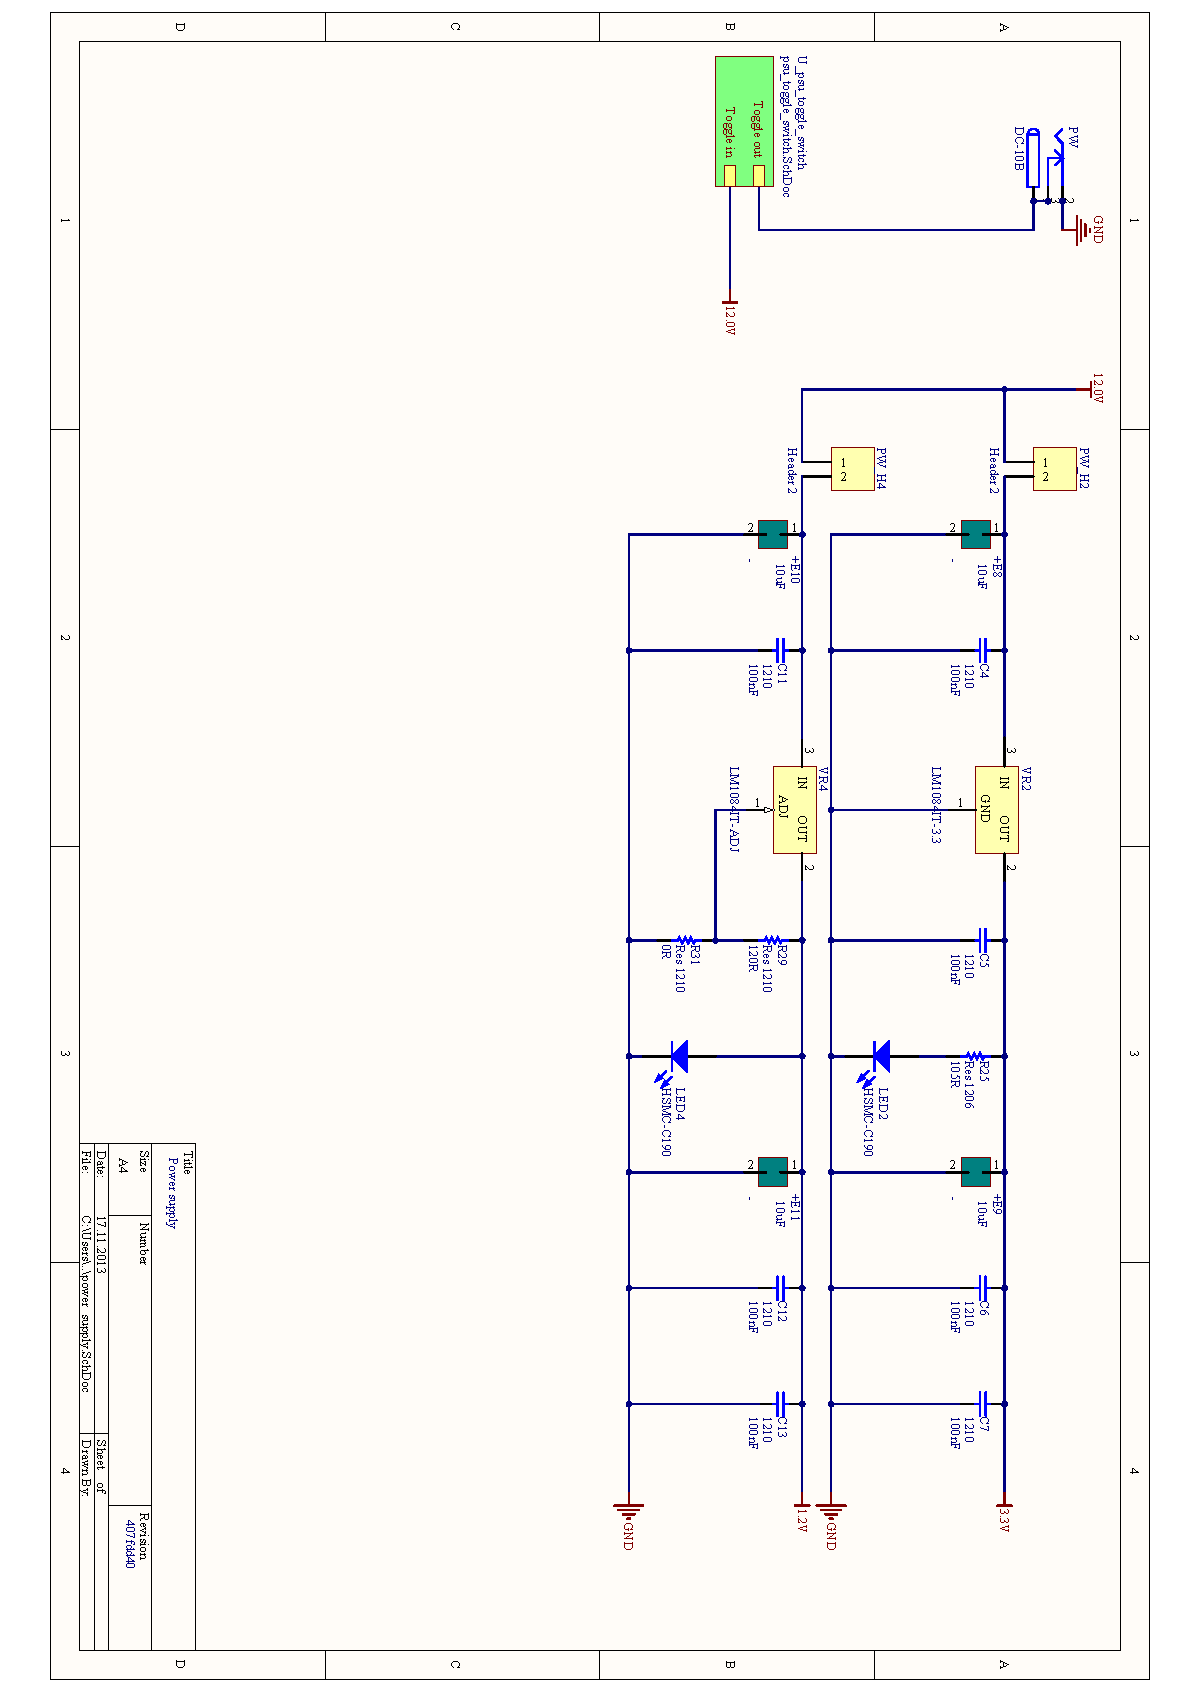
\includepdf[pages=-]{appendix/PCB_TDT4295_NTNU_2013_rotated.12.pdf}
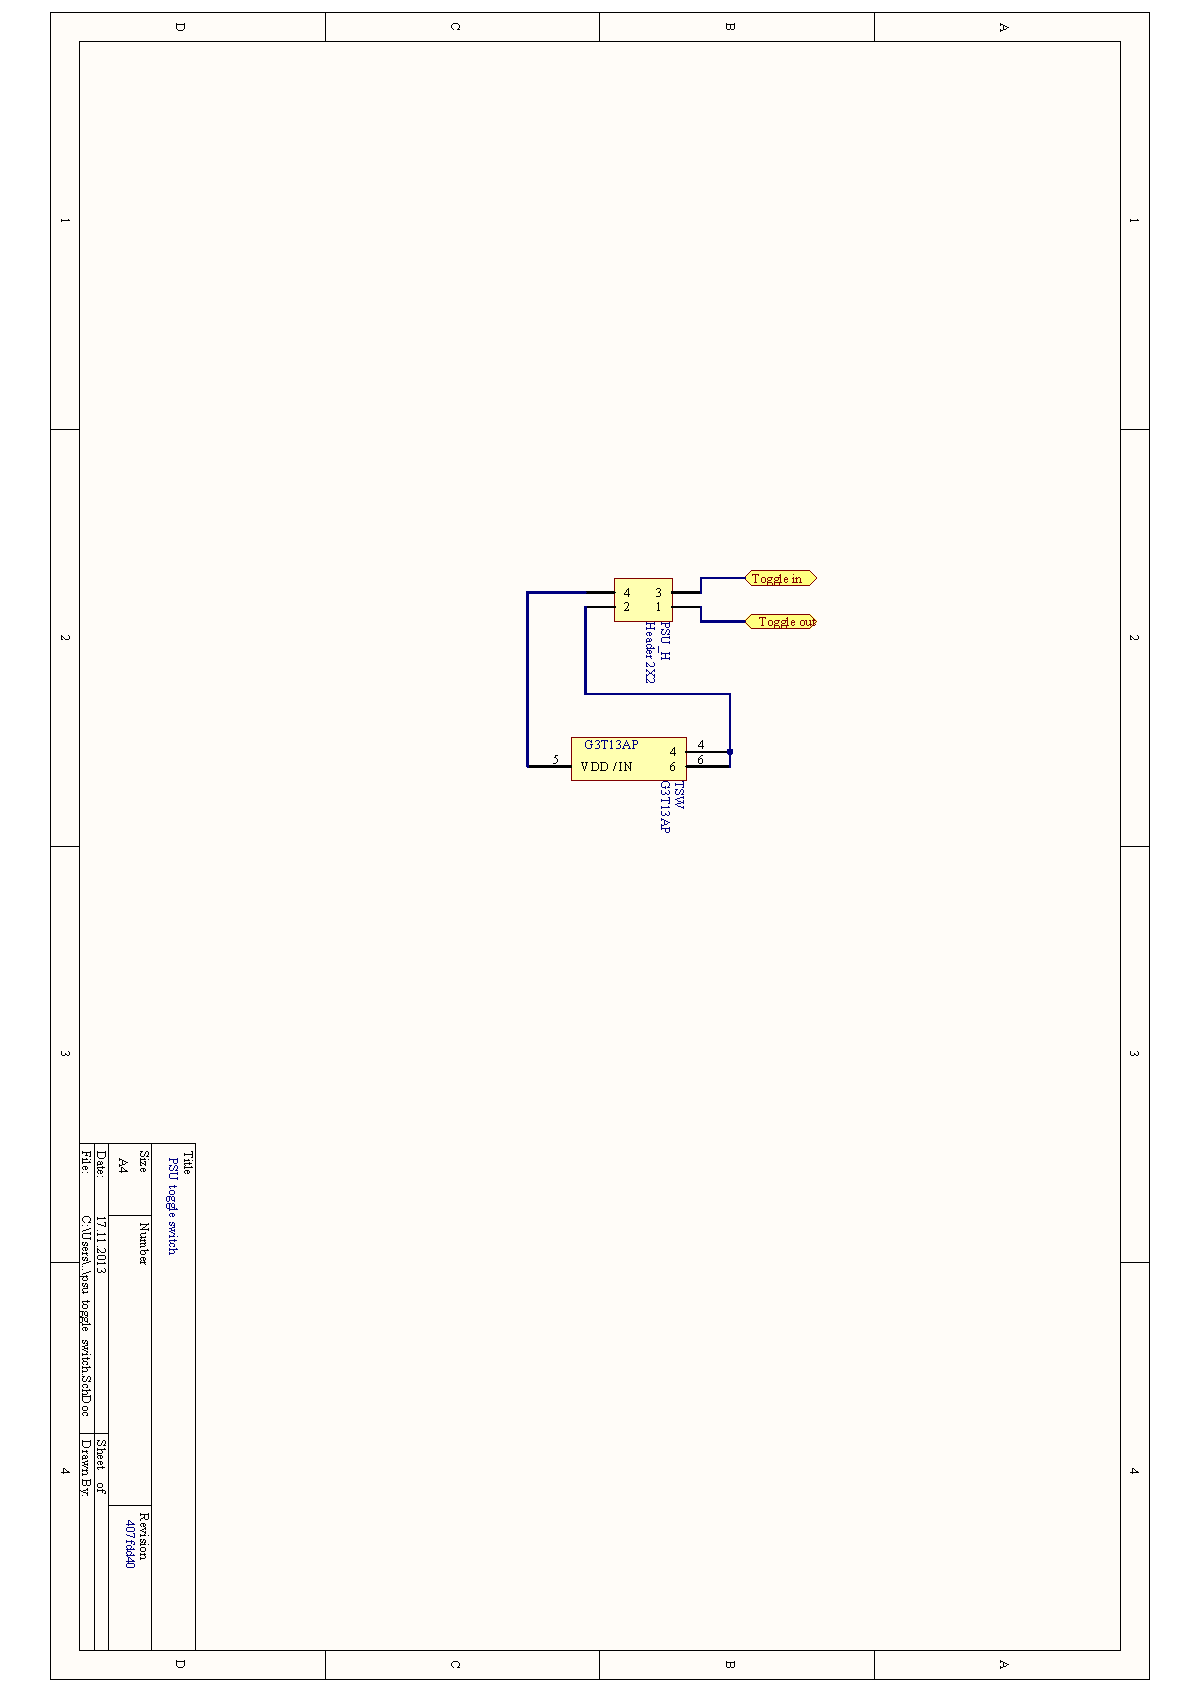
\includepdf[pages=-]{appendix/PCB_TDT4295_NTNU_2013_rotated.13.pdf}
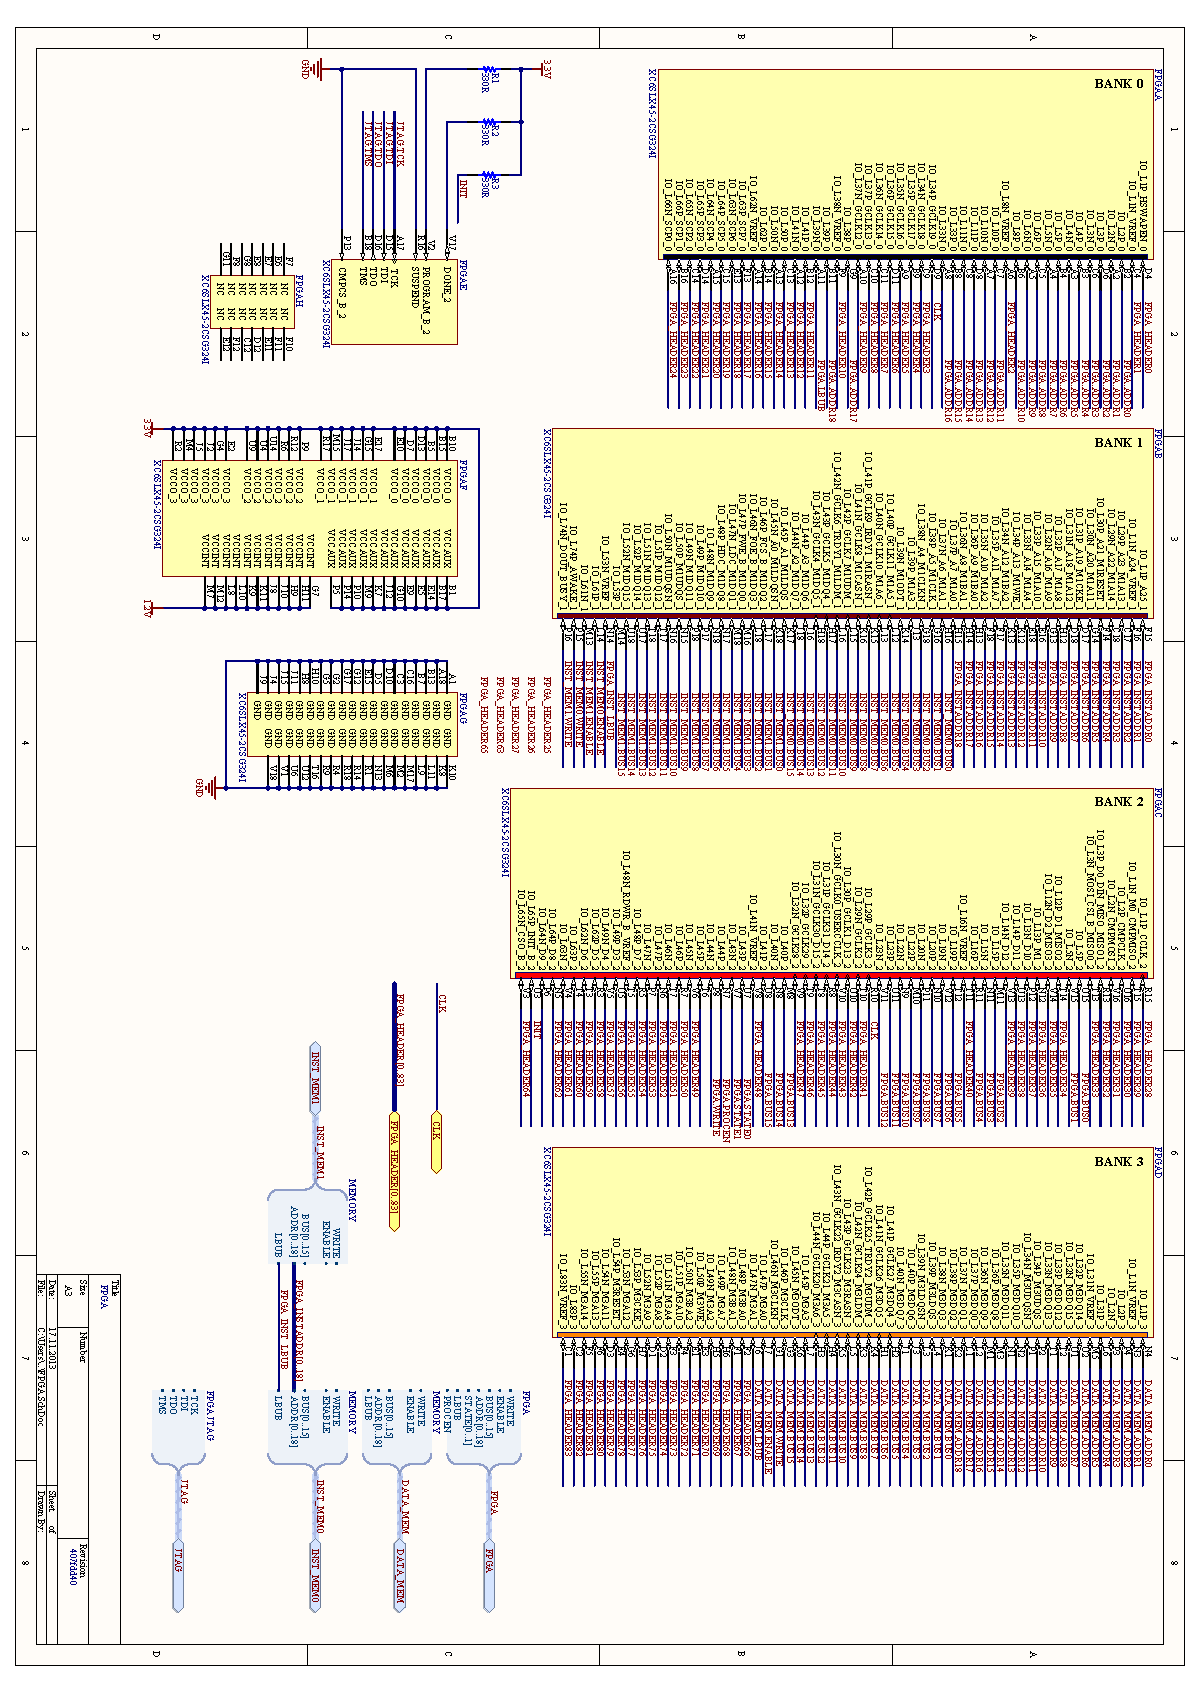
\includepdf[pages=-]{appendix/PCB_TDT4295_NTNU_2013_rotated.4.pdf}
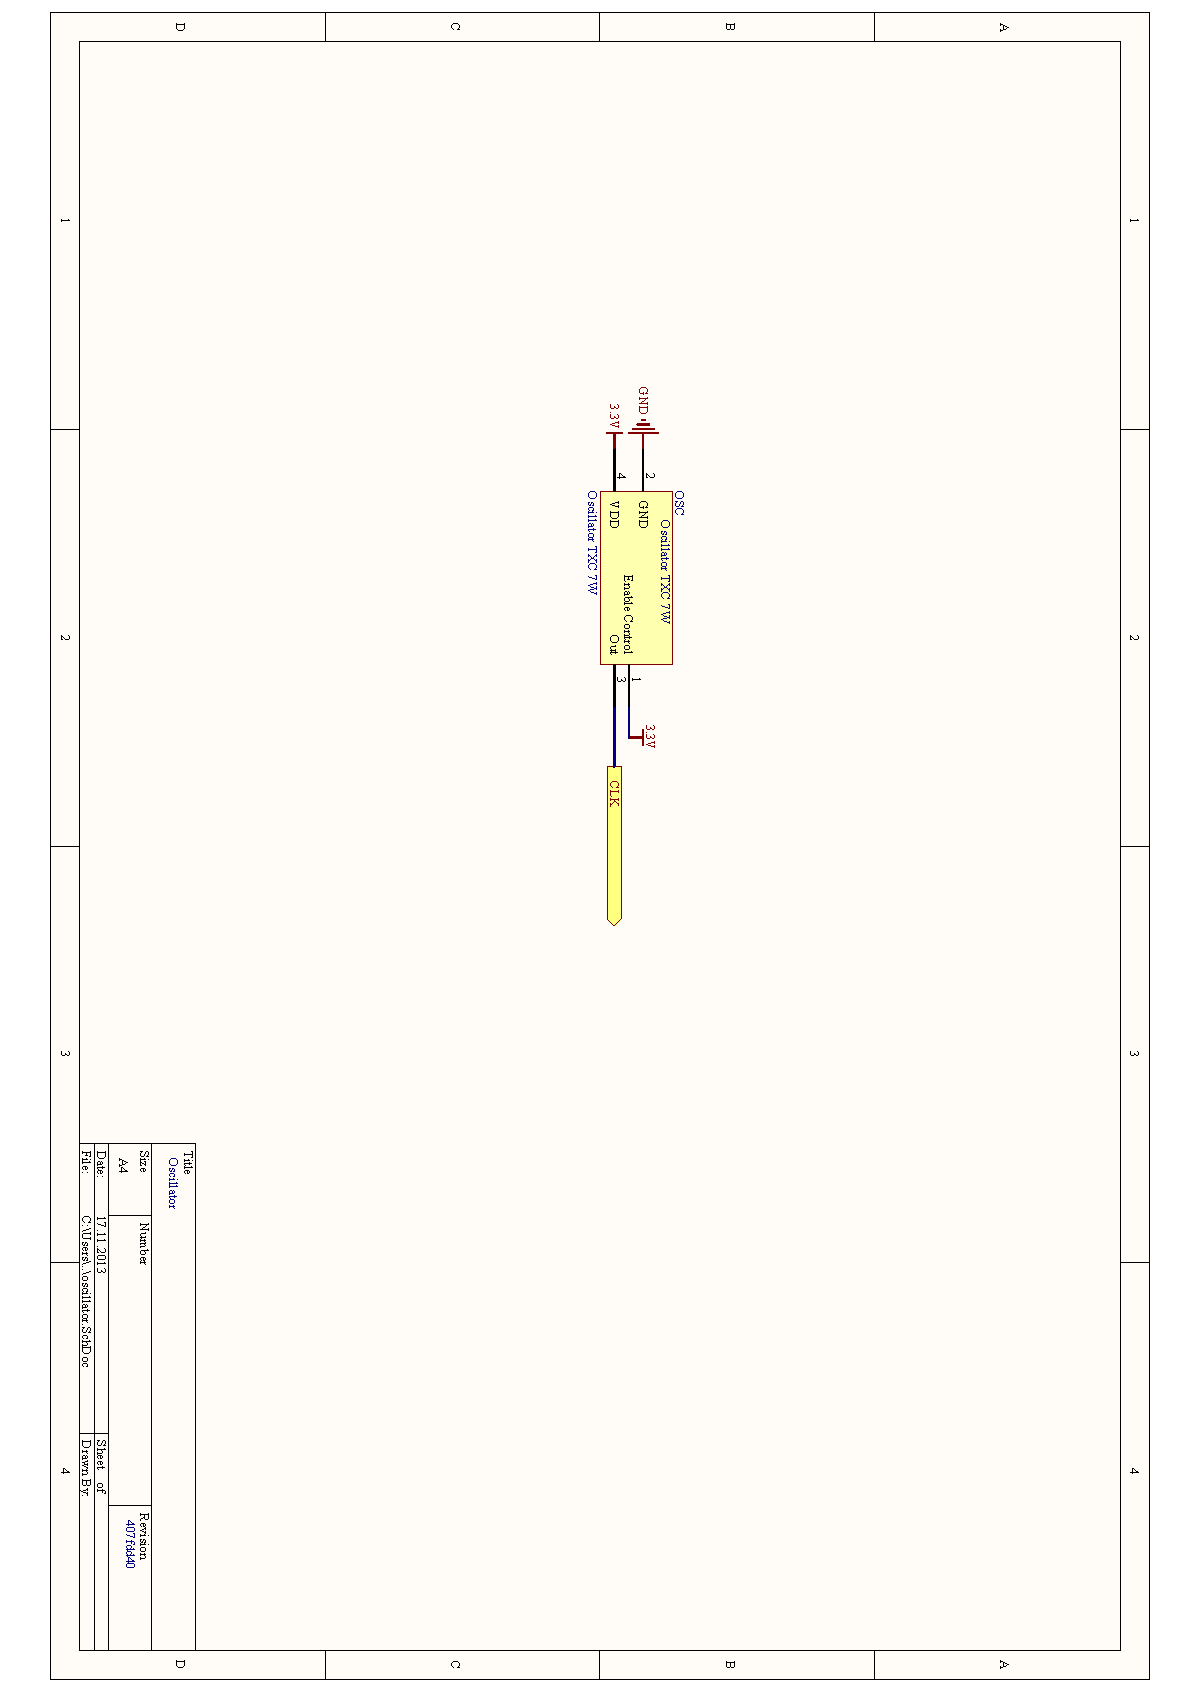
\includepdf[pages=-]{appendix/PCB_TDT4295_NTNU_2013_rotated.11.pdf}
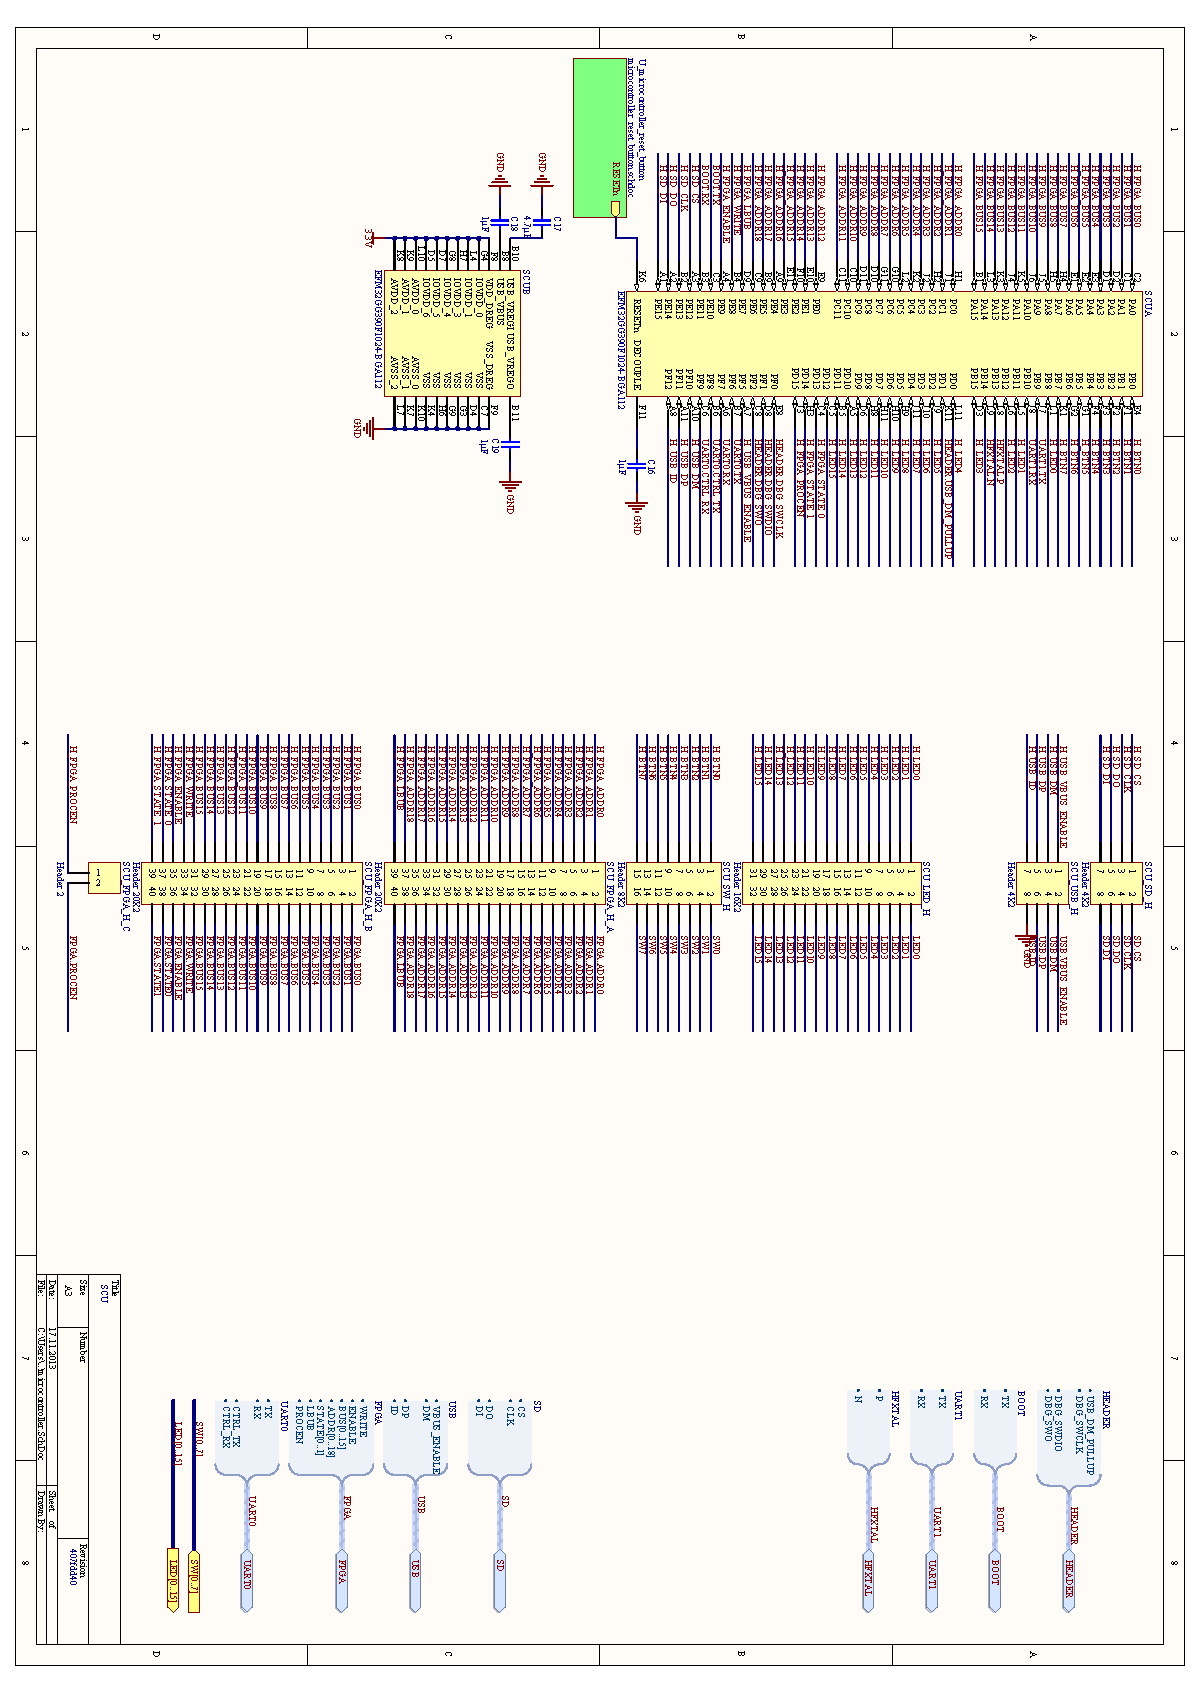
\includepdf[pages=-]{appendix/PCB_TDT4295_NTNU_2013_rotated.9.pdf}
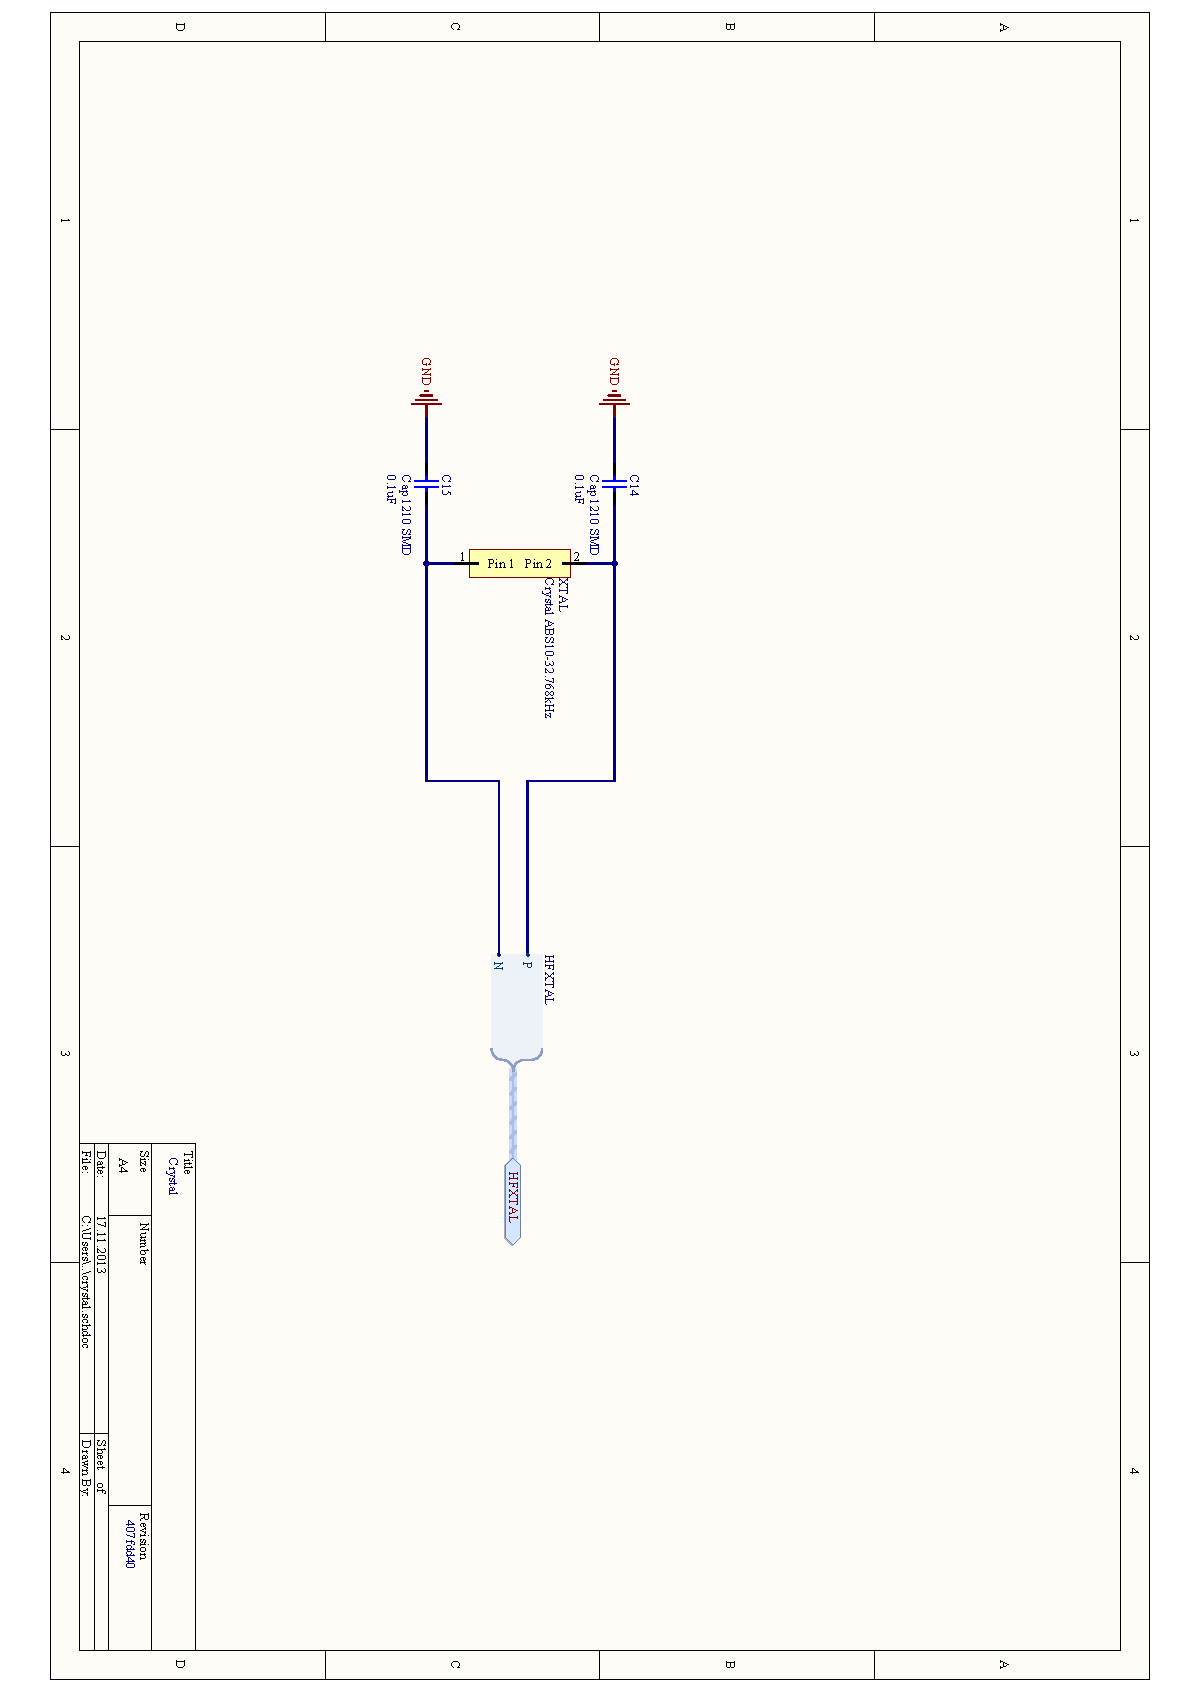
\includepdf[pages=-]{appendix/PCB_TDT4295_NTNU_2013_rotated.2.pdf}
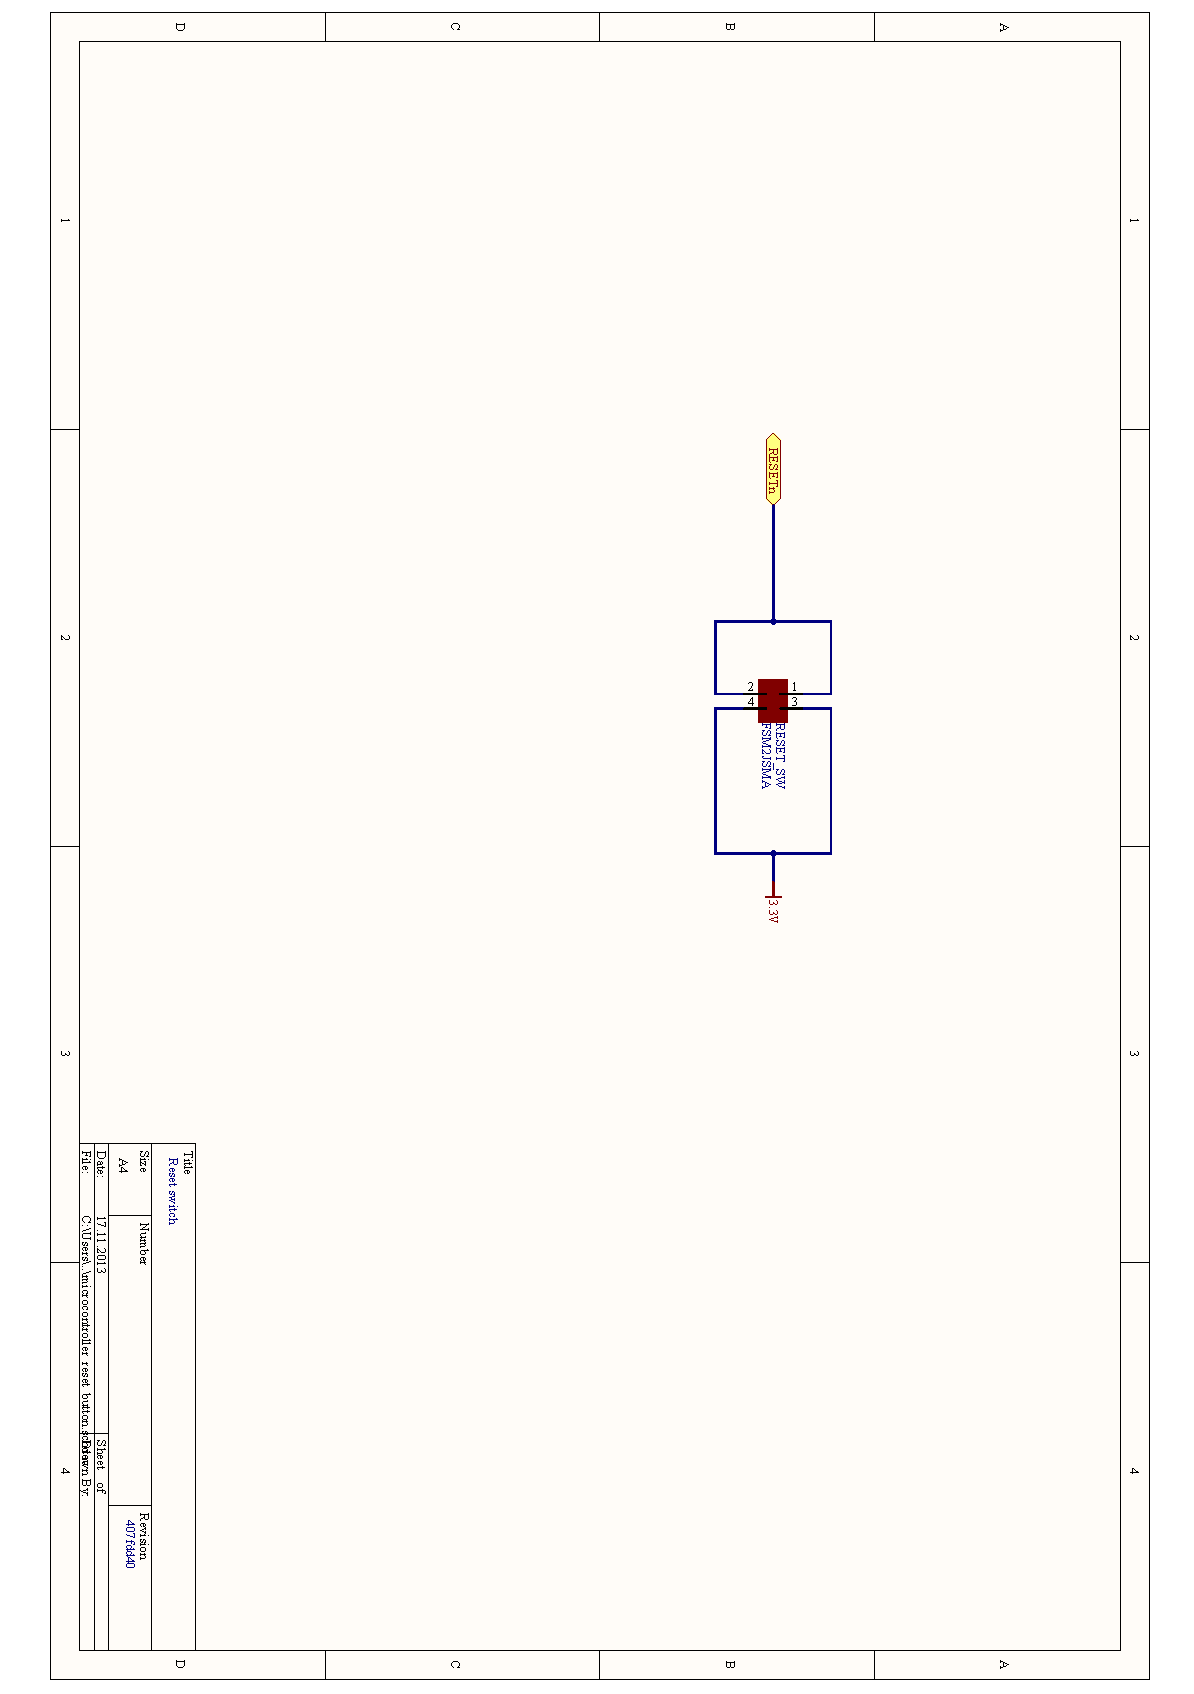
\includepdf[pages=-]{appendix/PCB_TDT4295_NTNU_2013_rotated.10.pdf}
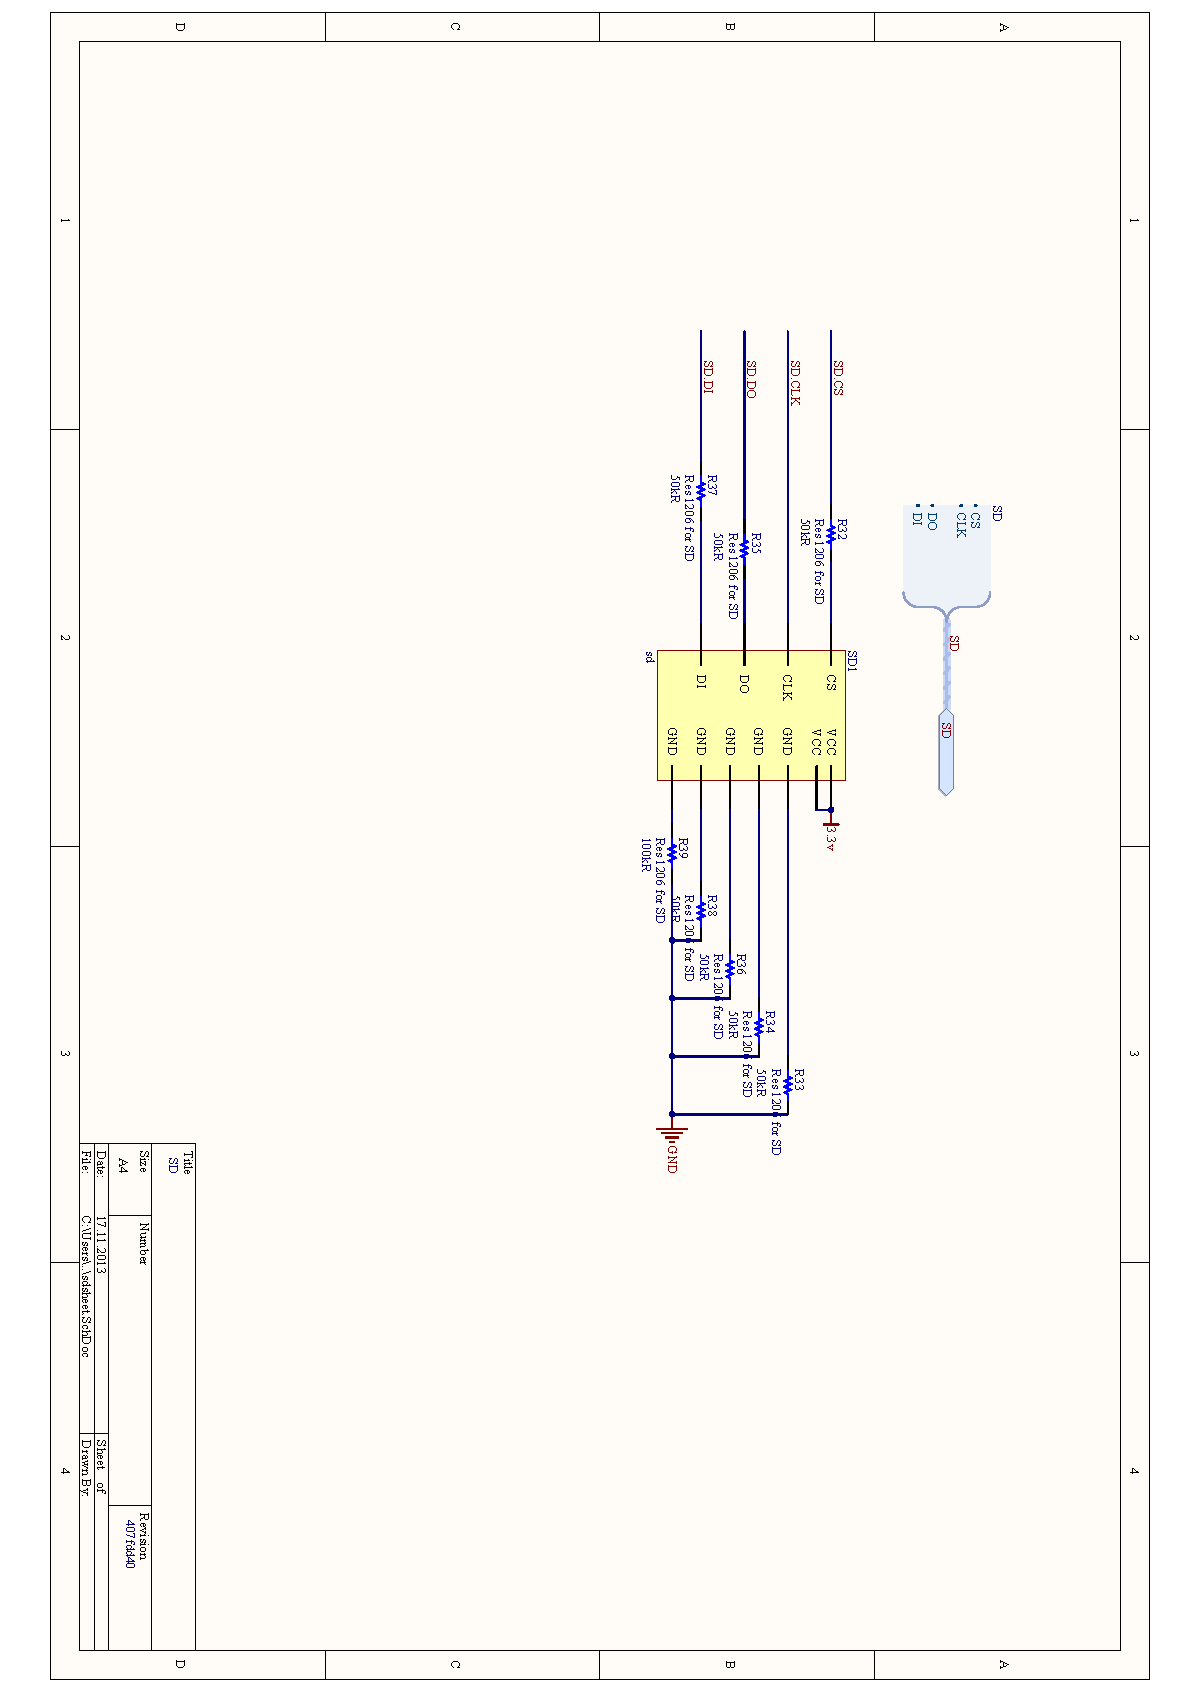
\includepdf[pages=-]{appendix/PCB_TDT4295_NTNU_2013_rotated.14.pdf}
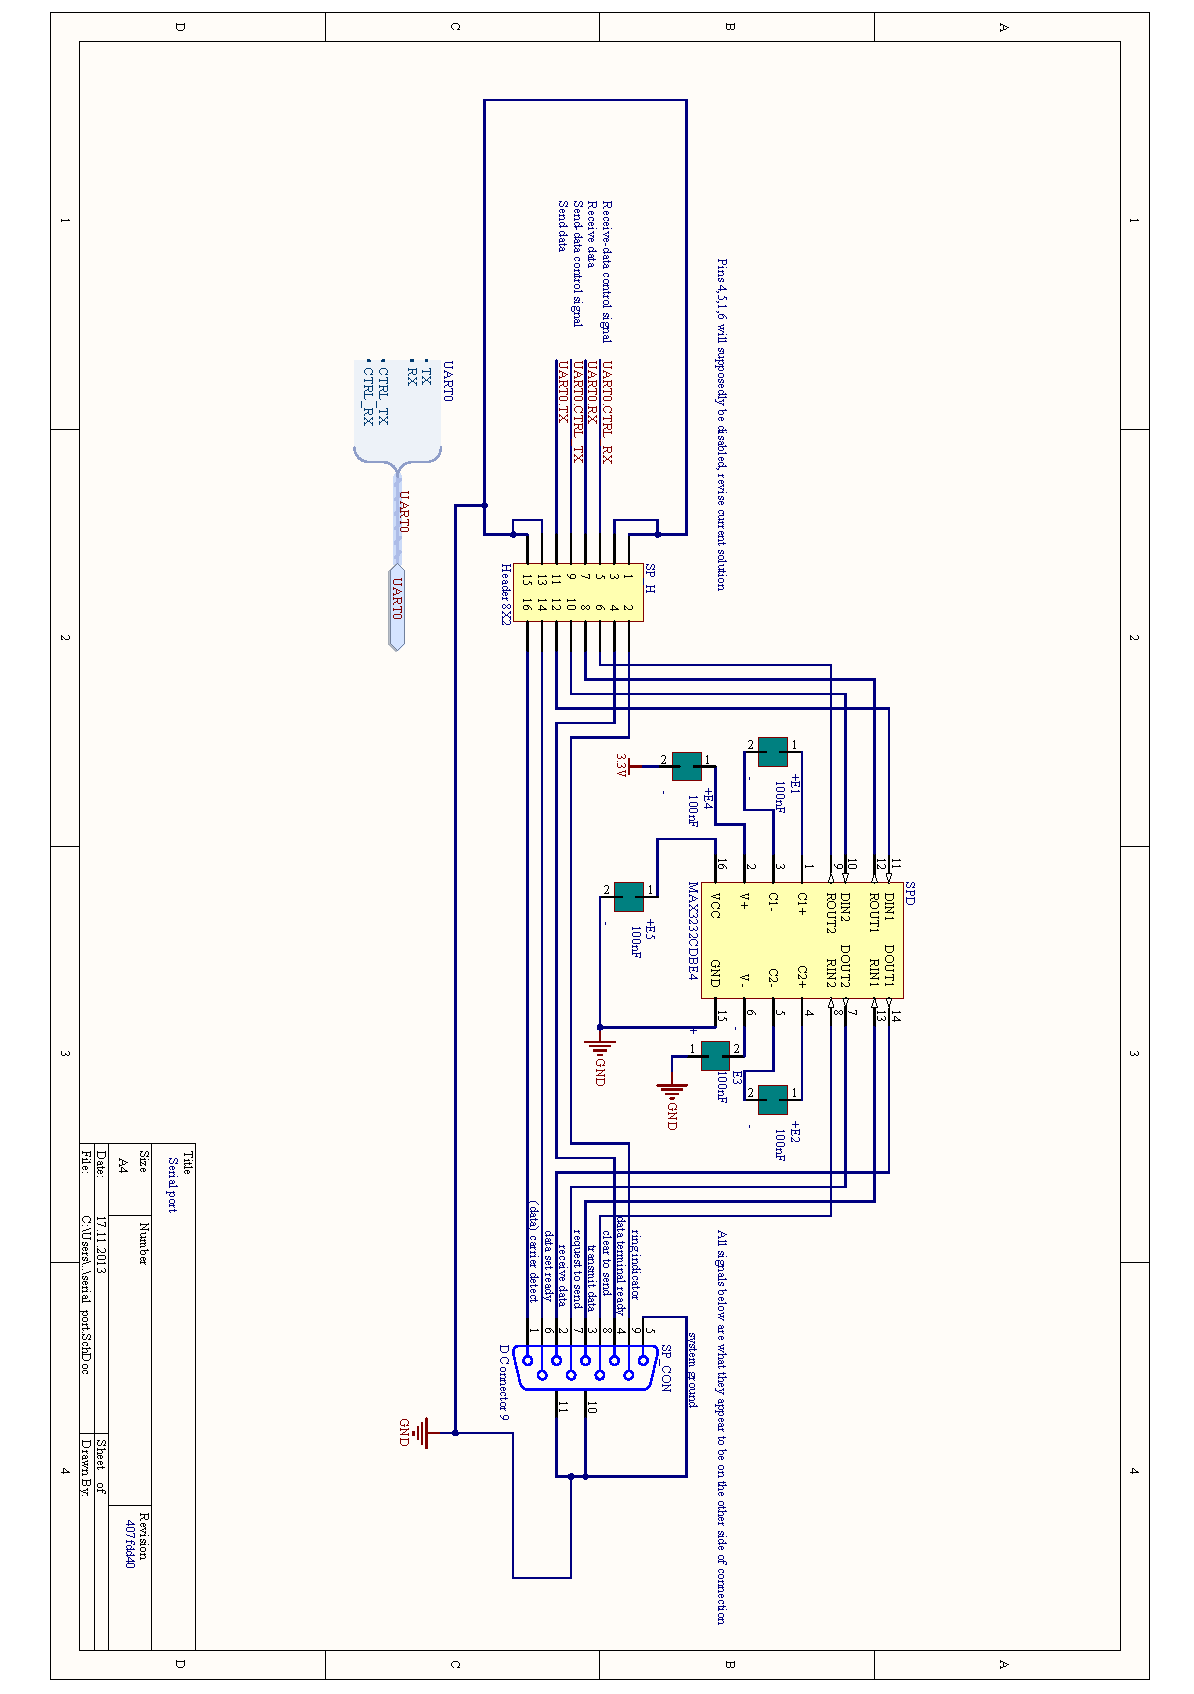
\includepdf[pages=-]{appendix/PCB_TDT4295_NTNU_2013_rotated.15.pdf}
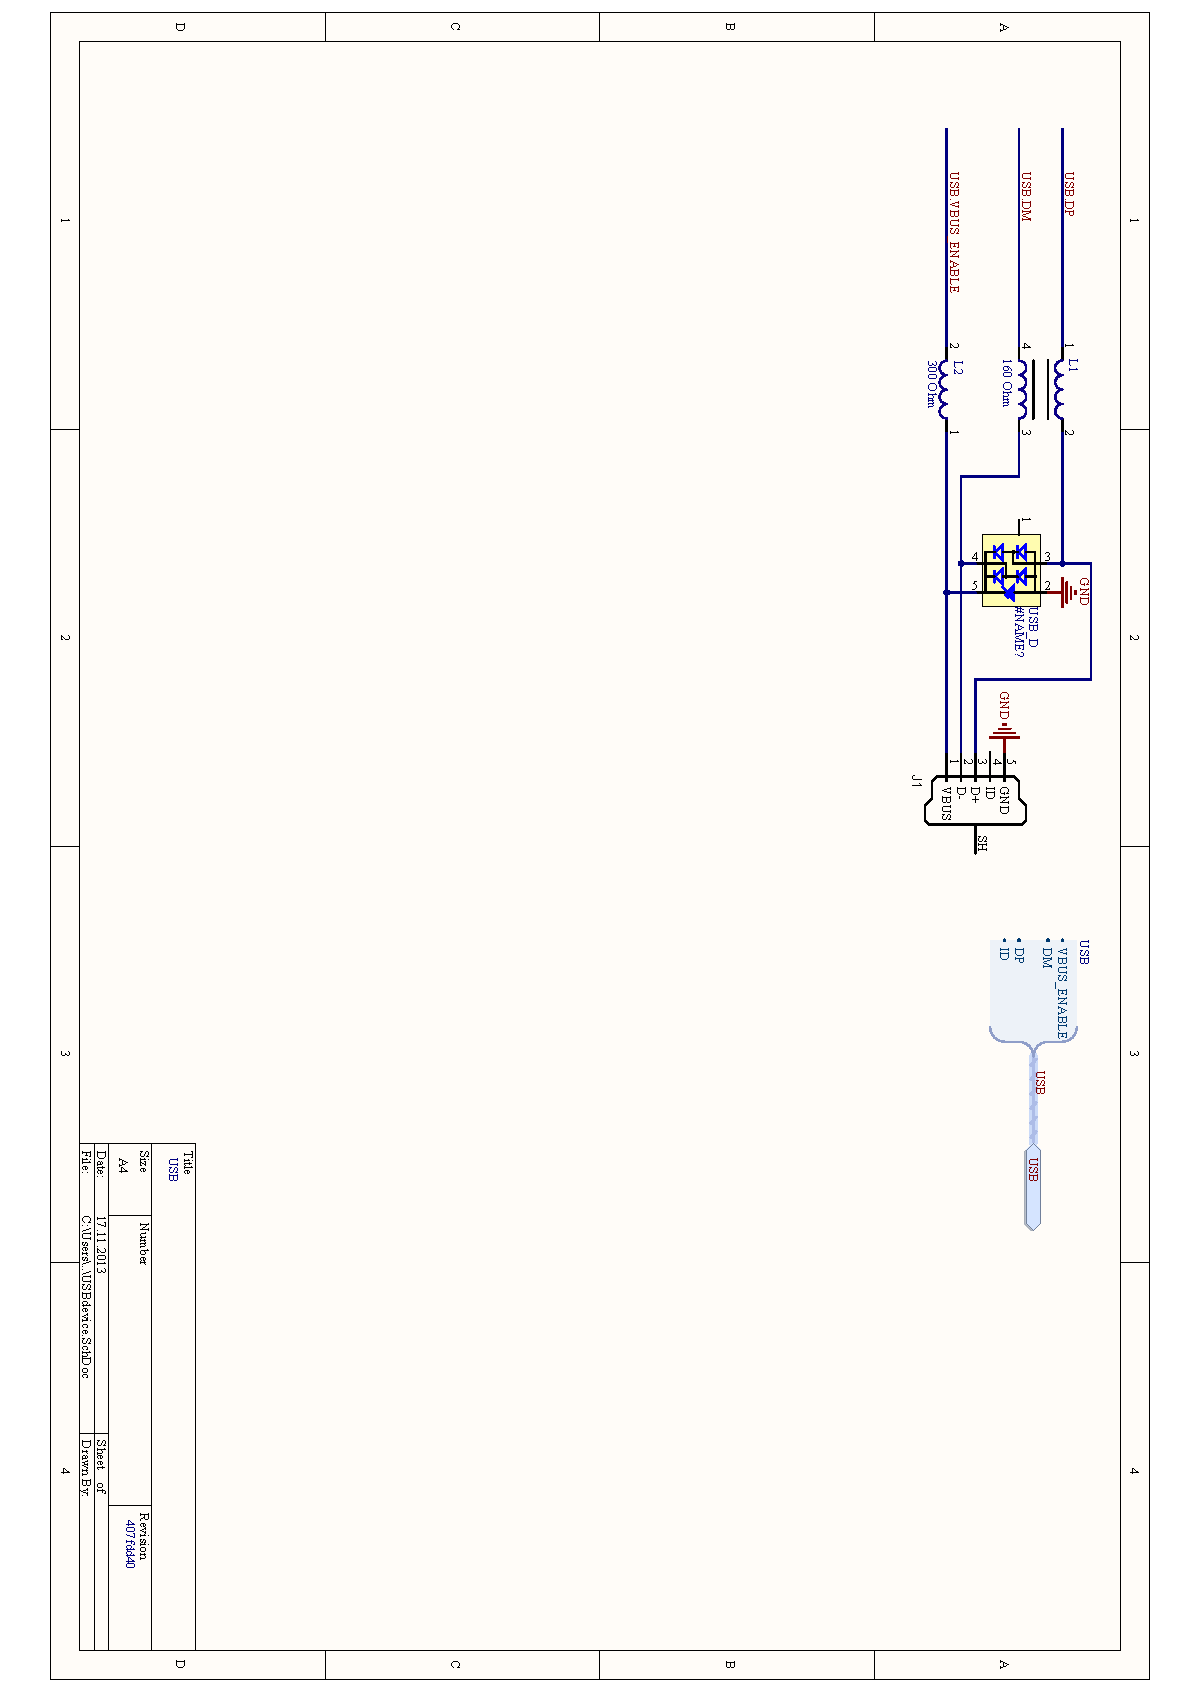
\includepdf[pages=-]{appendix/PCB_TDT4295_NTNU_2013_rotated.17.pdf}
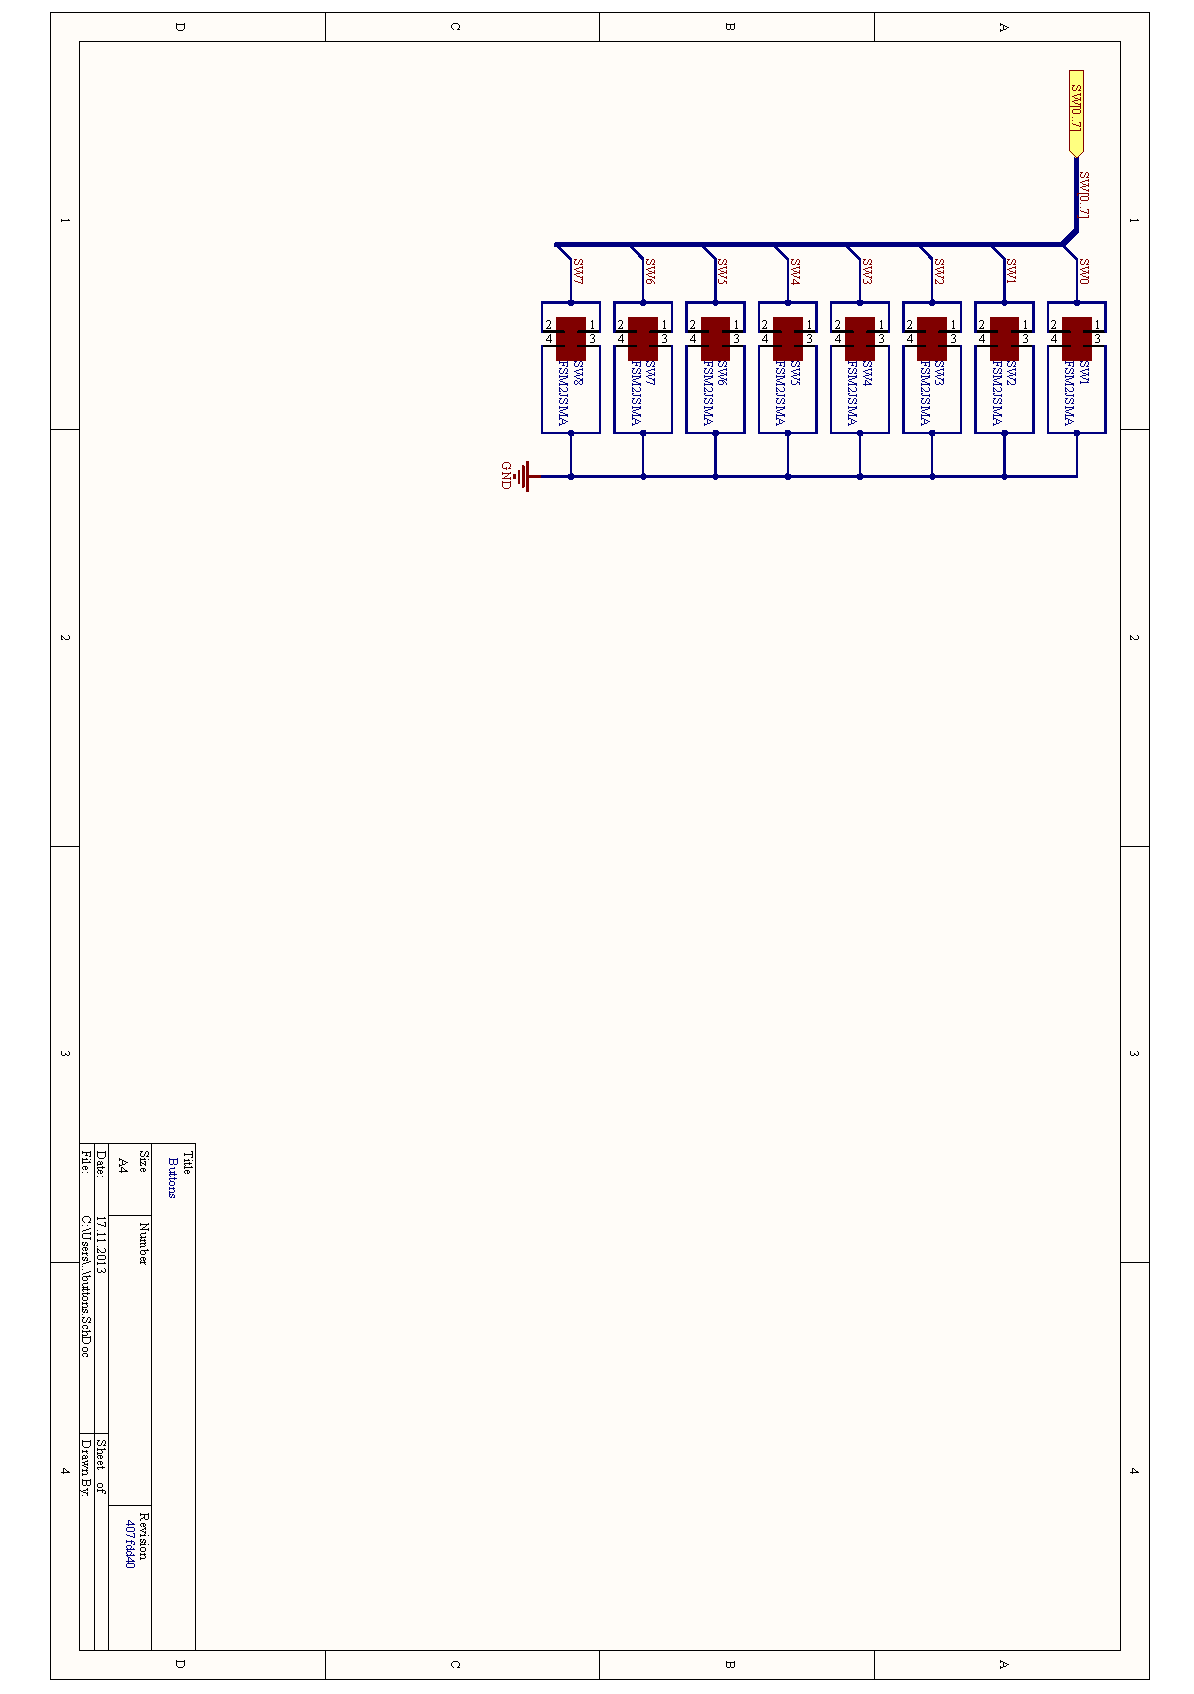
\includepdf[pages=-]{appendix/PCB_TDT4295_NTNU_2013_rotated.1.pdf}
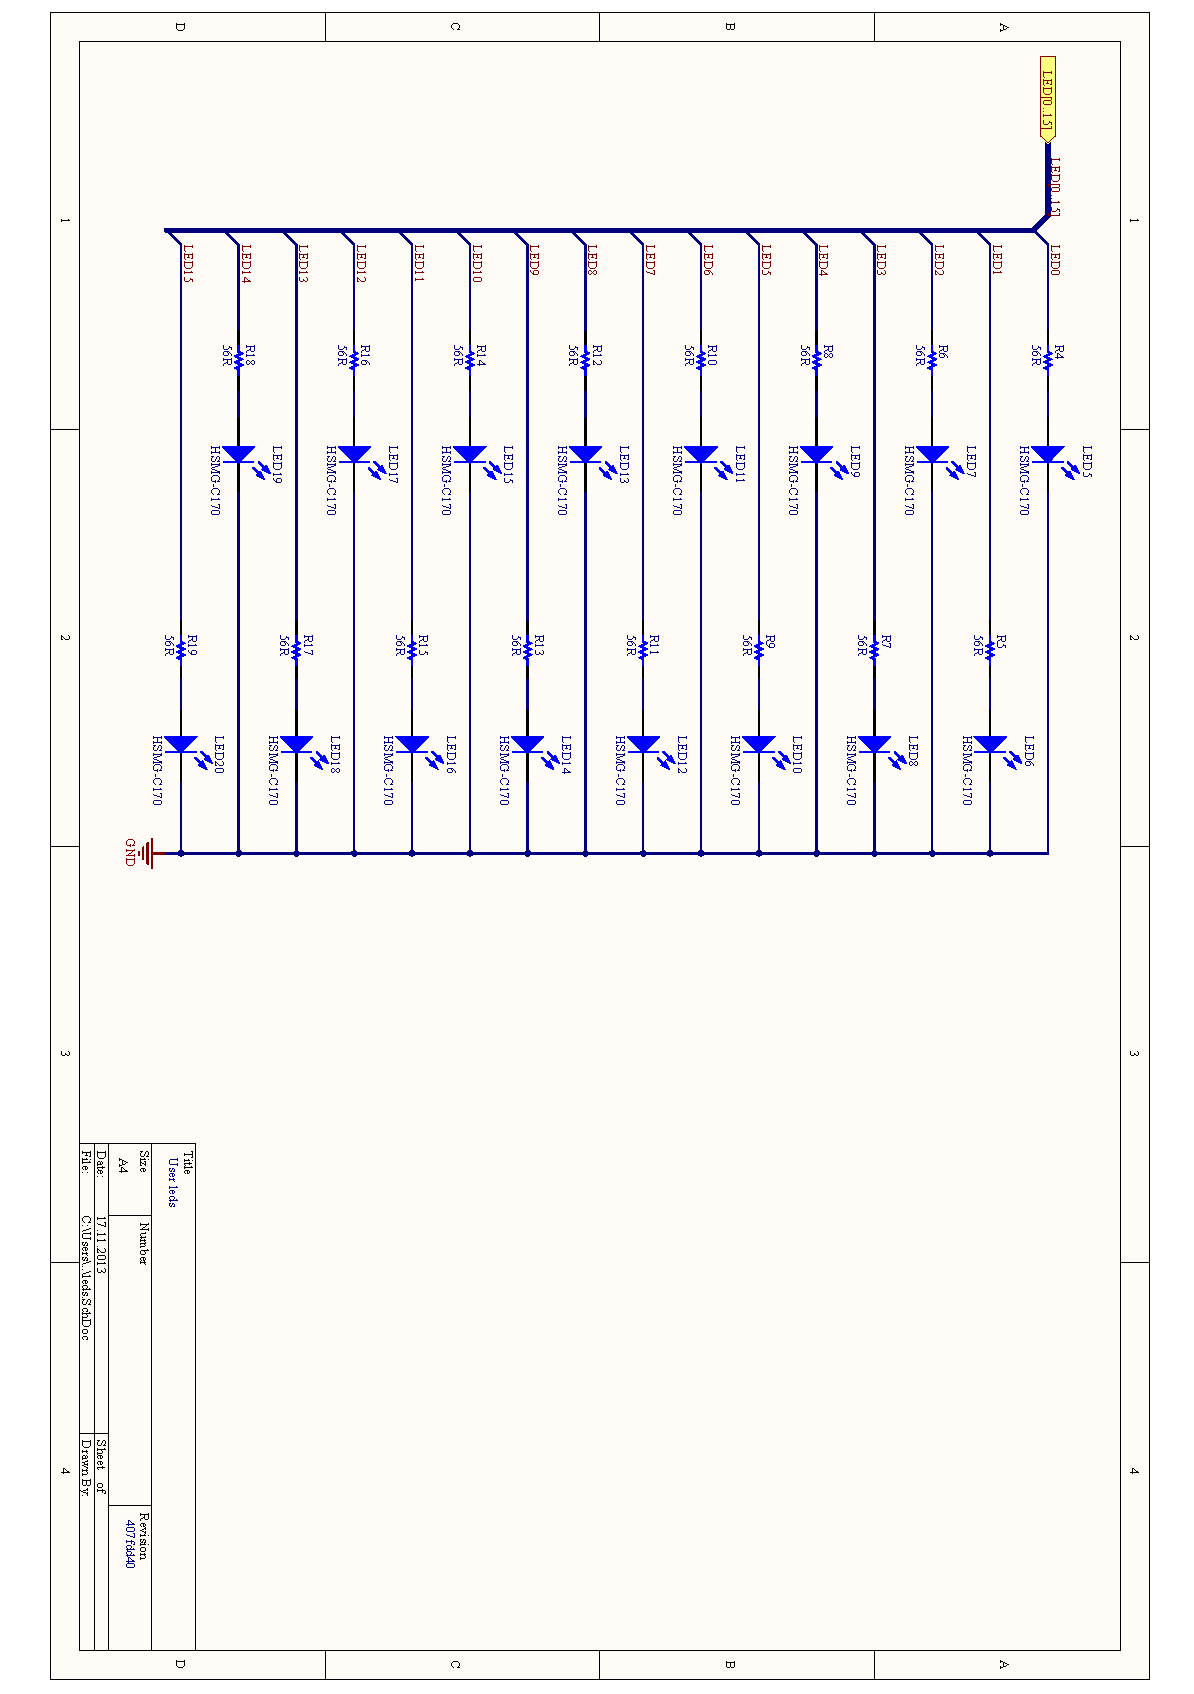
\includepdf[pages=-]{appendix/PCB_TDT4295_NTNU_2013_rotated.6.pdf}
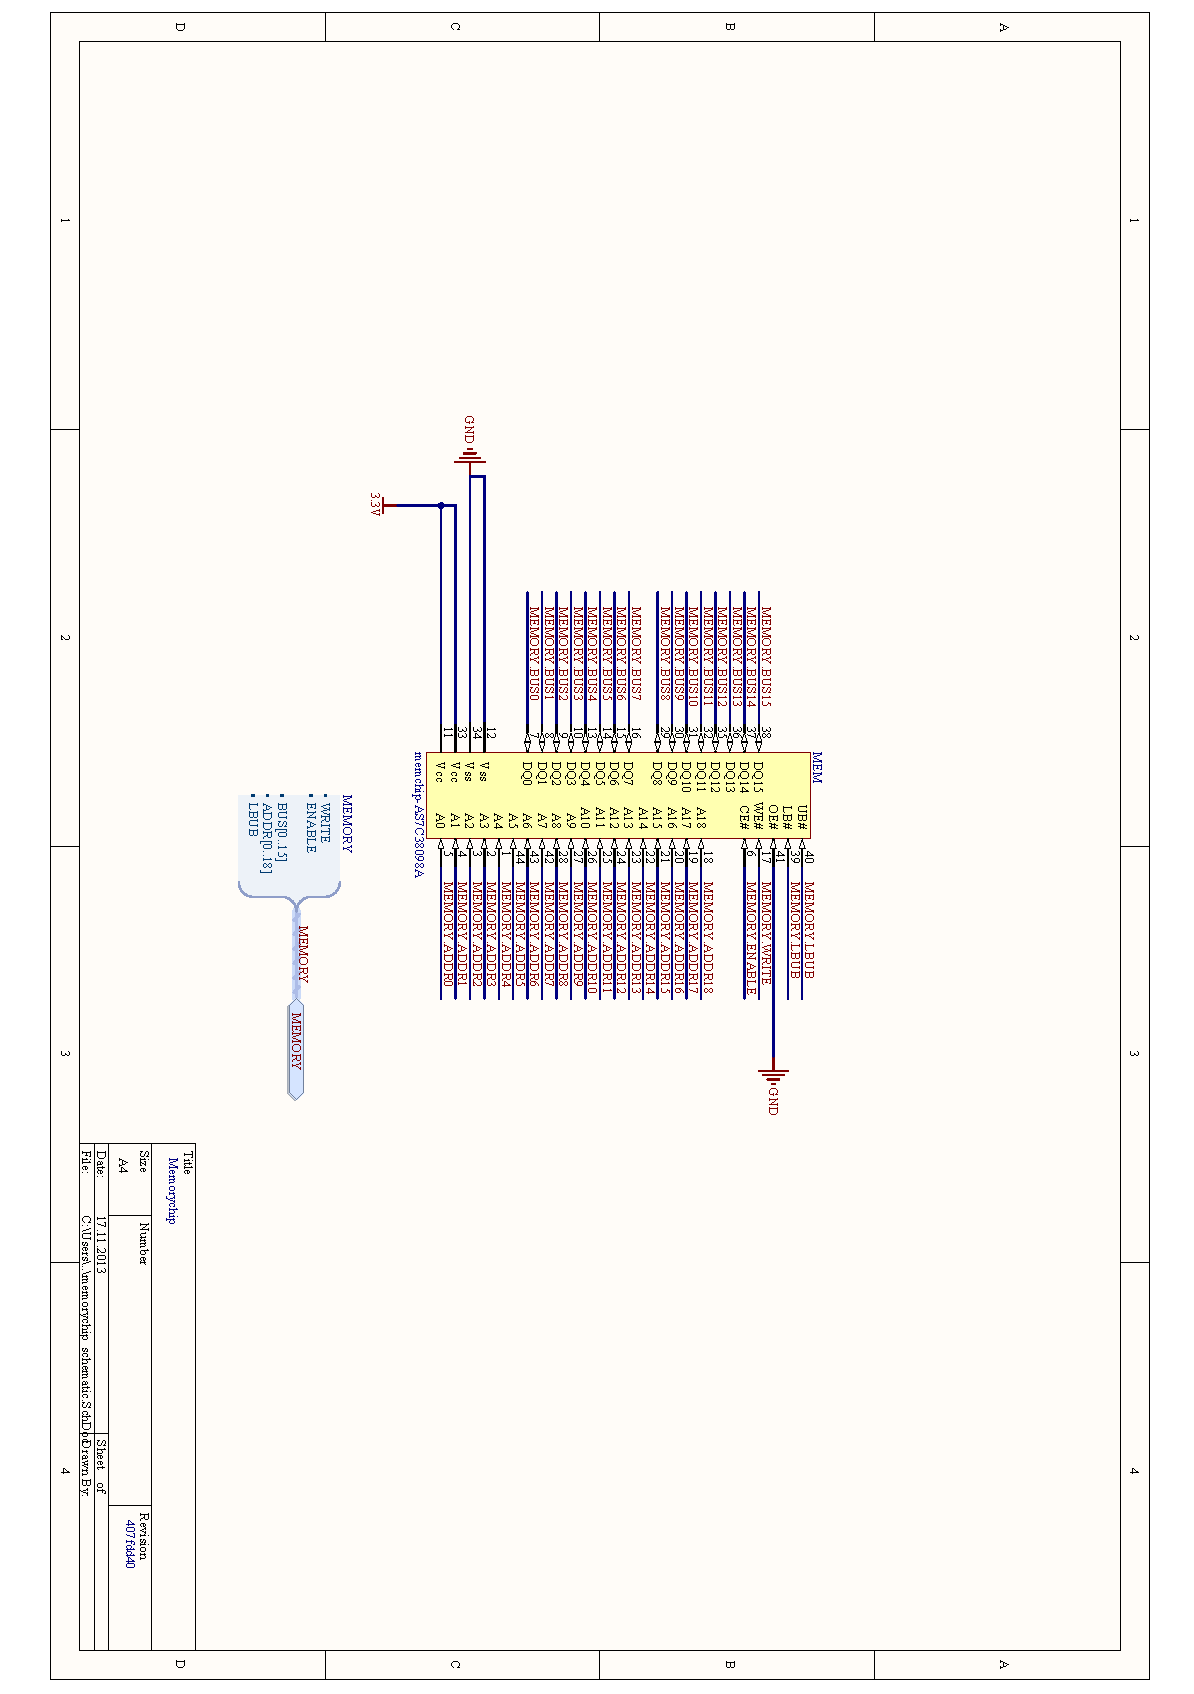
\includepdf[pages=-]{appendix/PCB_TDT4295_NTNU_2013_rotated.8.pdf}
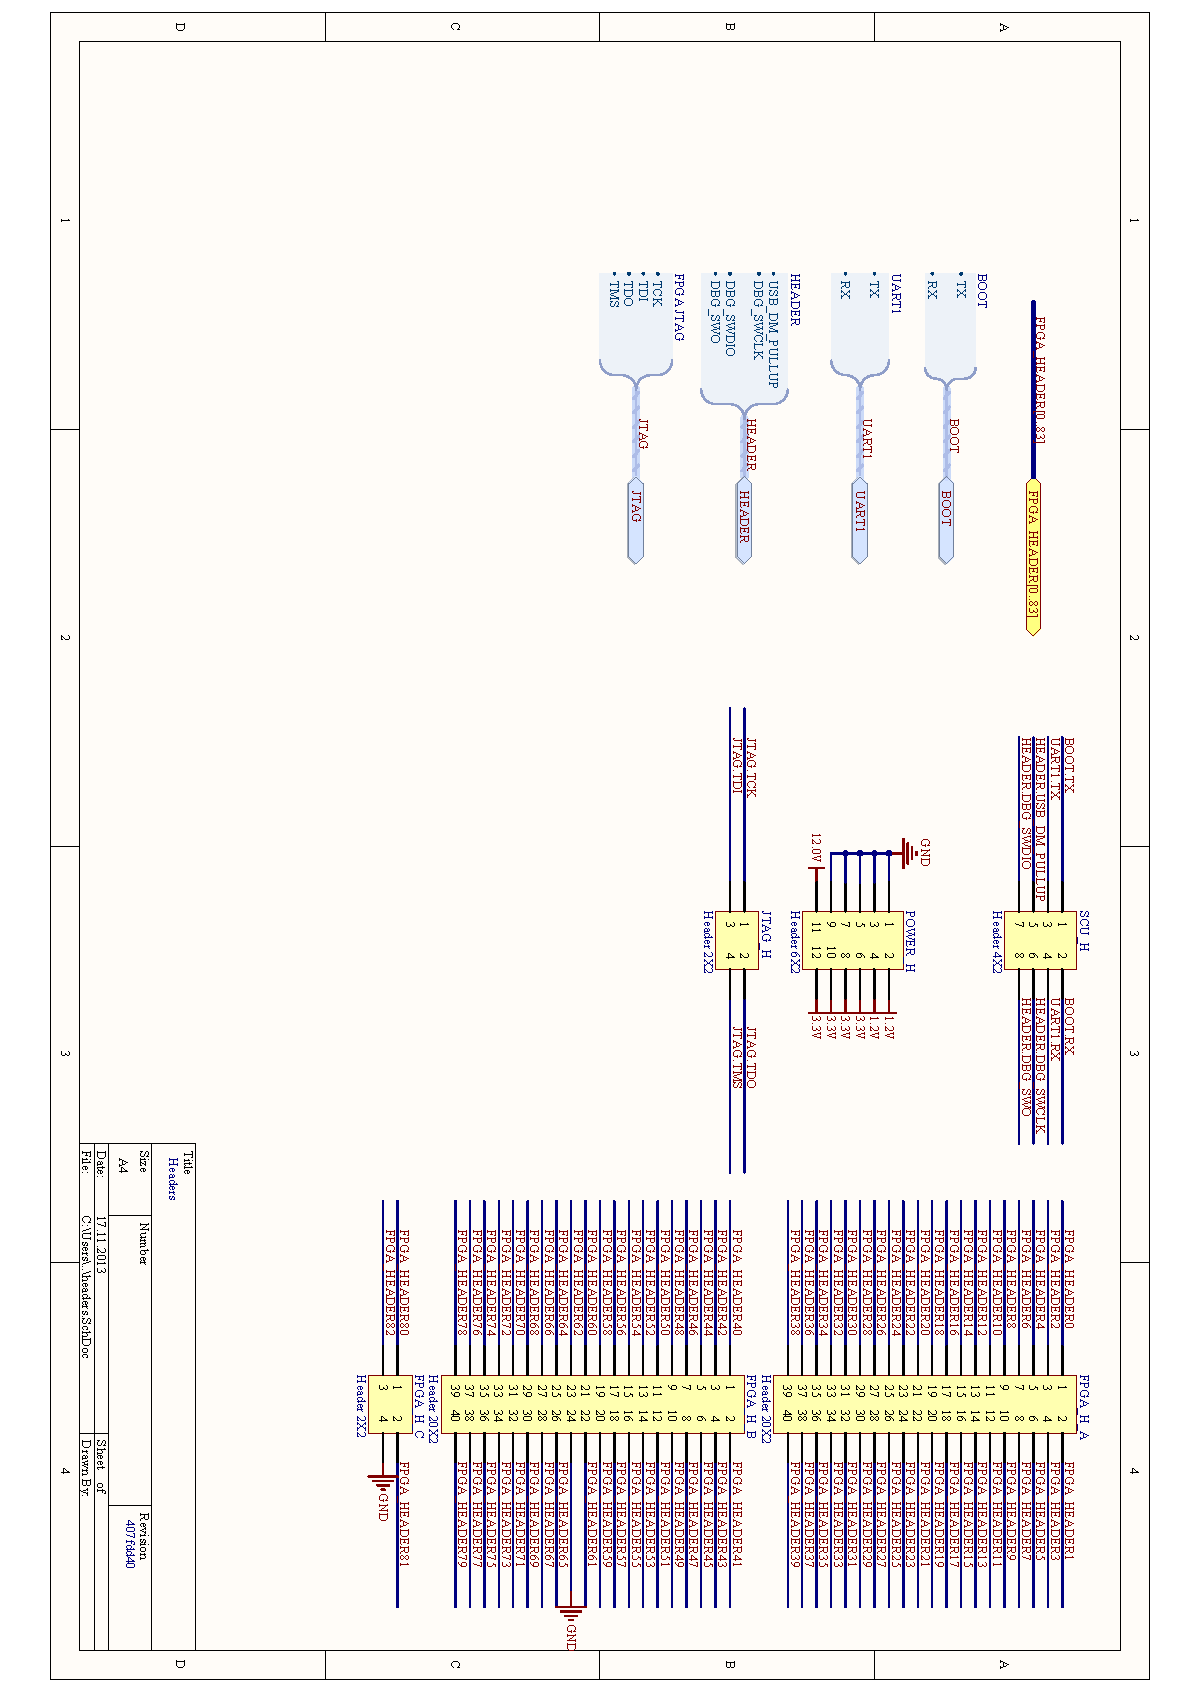
\includepdf[pages=-]{appendix/PCB_TDT4295_NTNU_2013_rotated.5.pdf}
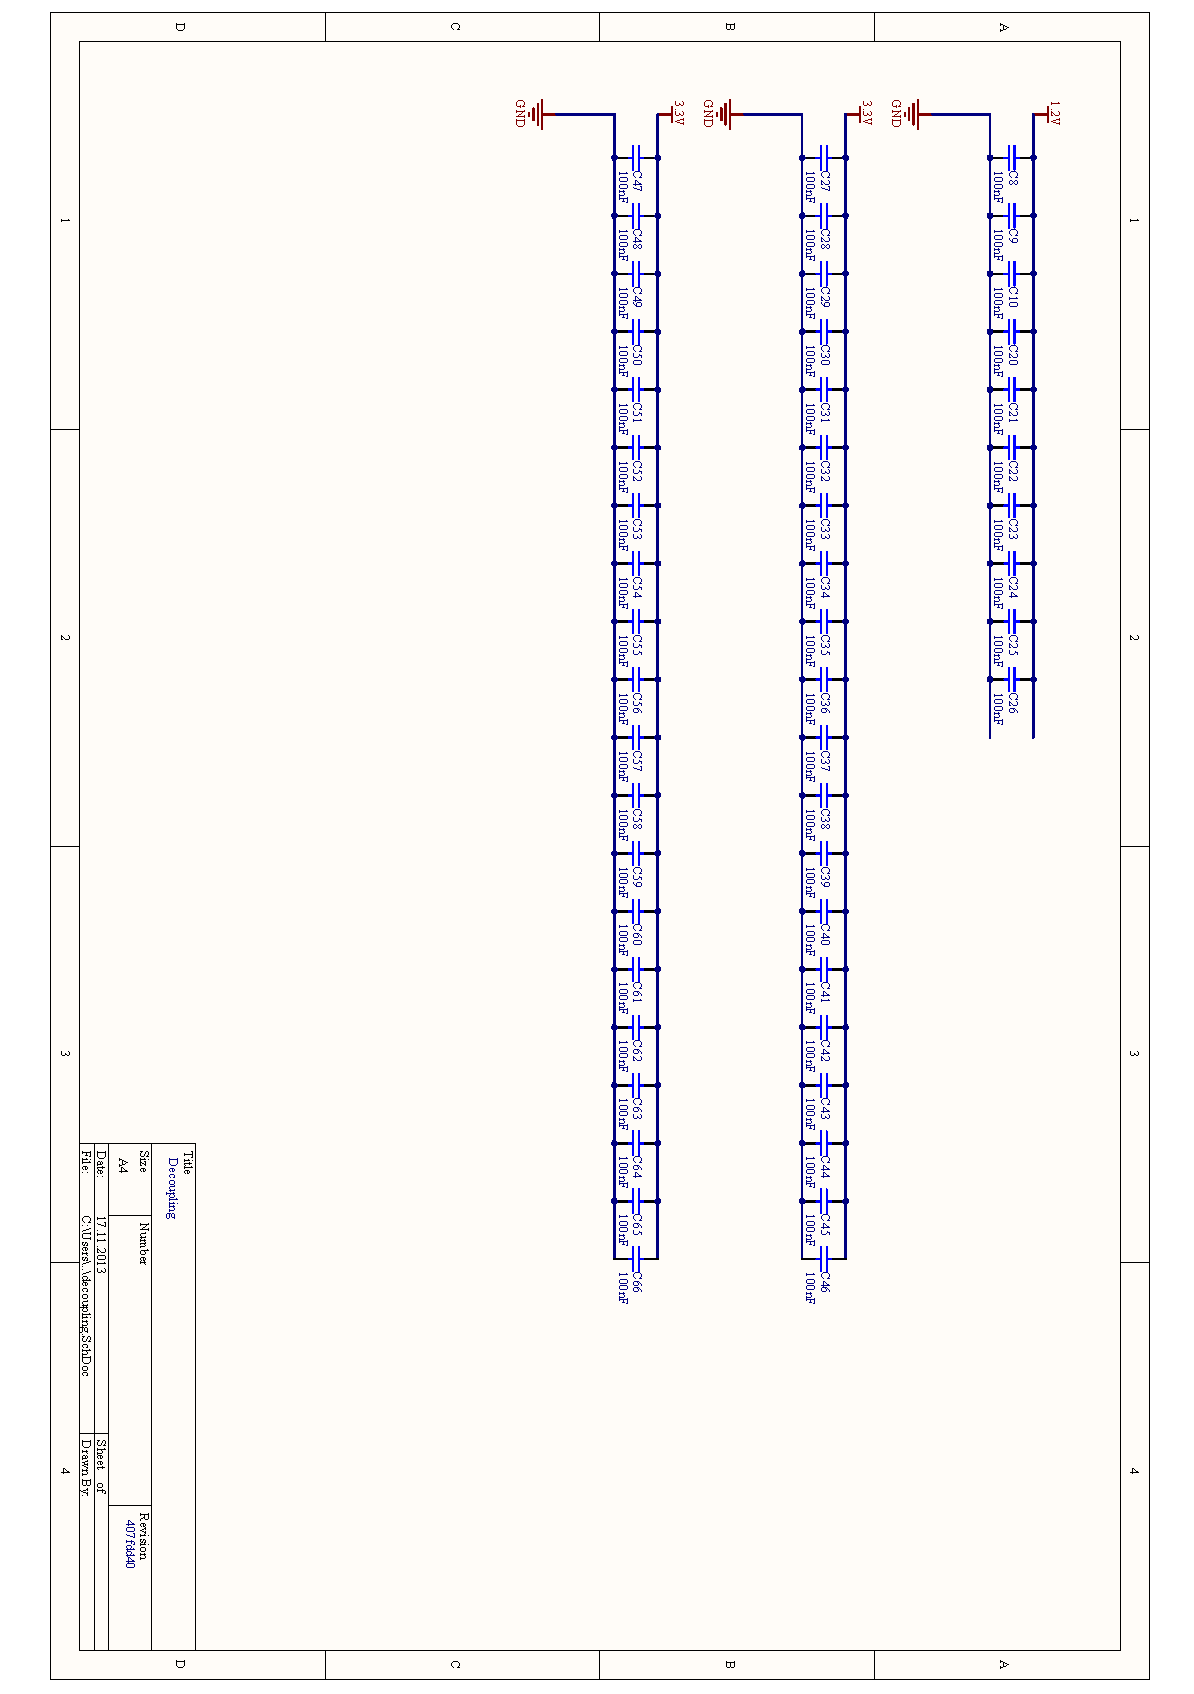
\includepdf[pages=-]{appendix/PCB_TDT4295_NTNU_2013_rotated.3.pdf}
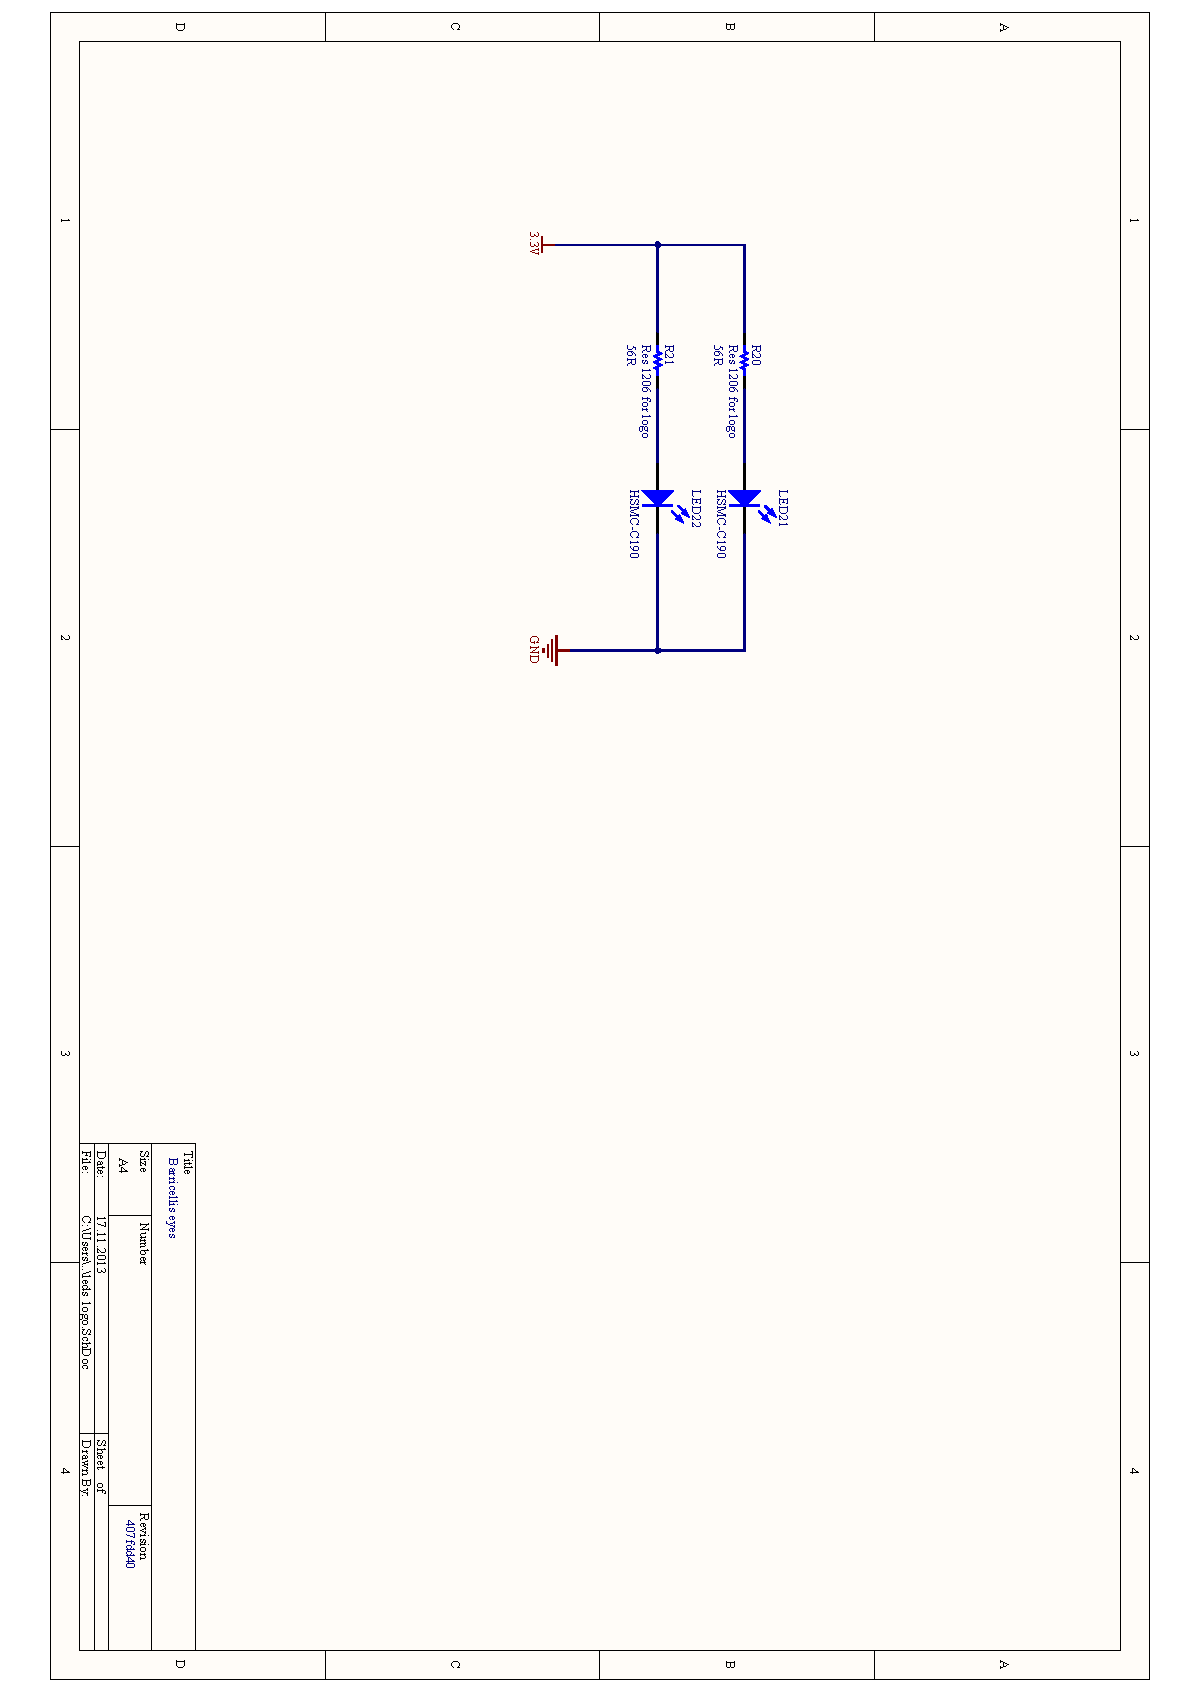
\includepdf[pages=-]{appendix/PCB_TDT4295_NTNU_2013_rotated.7.pdf}
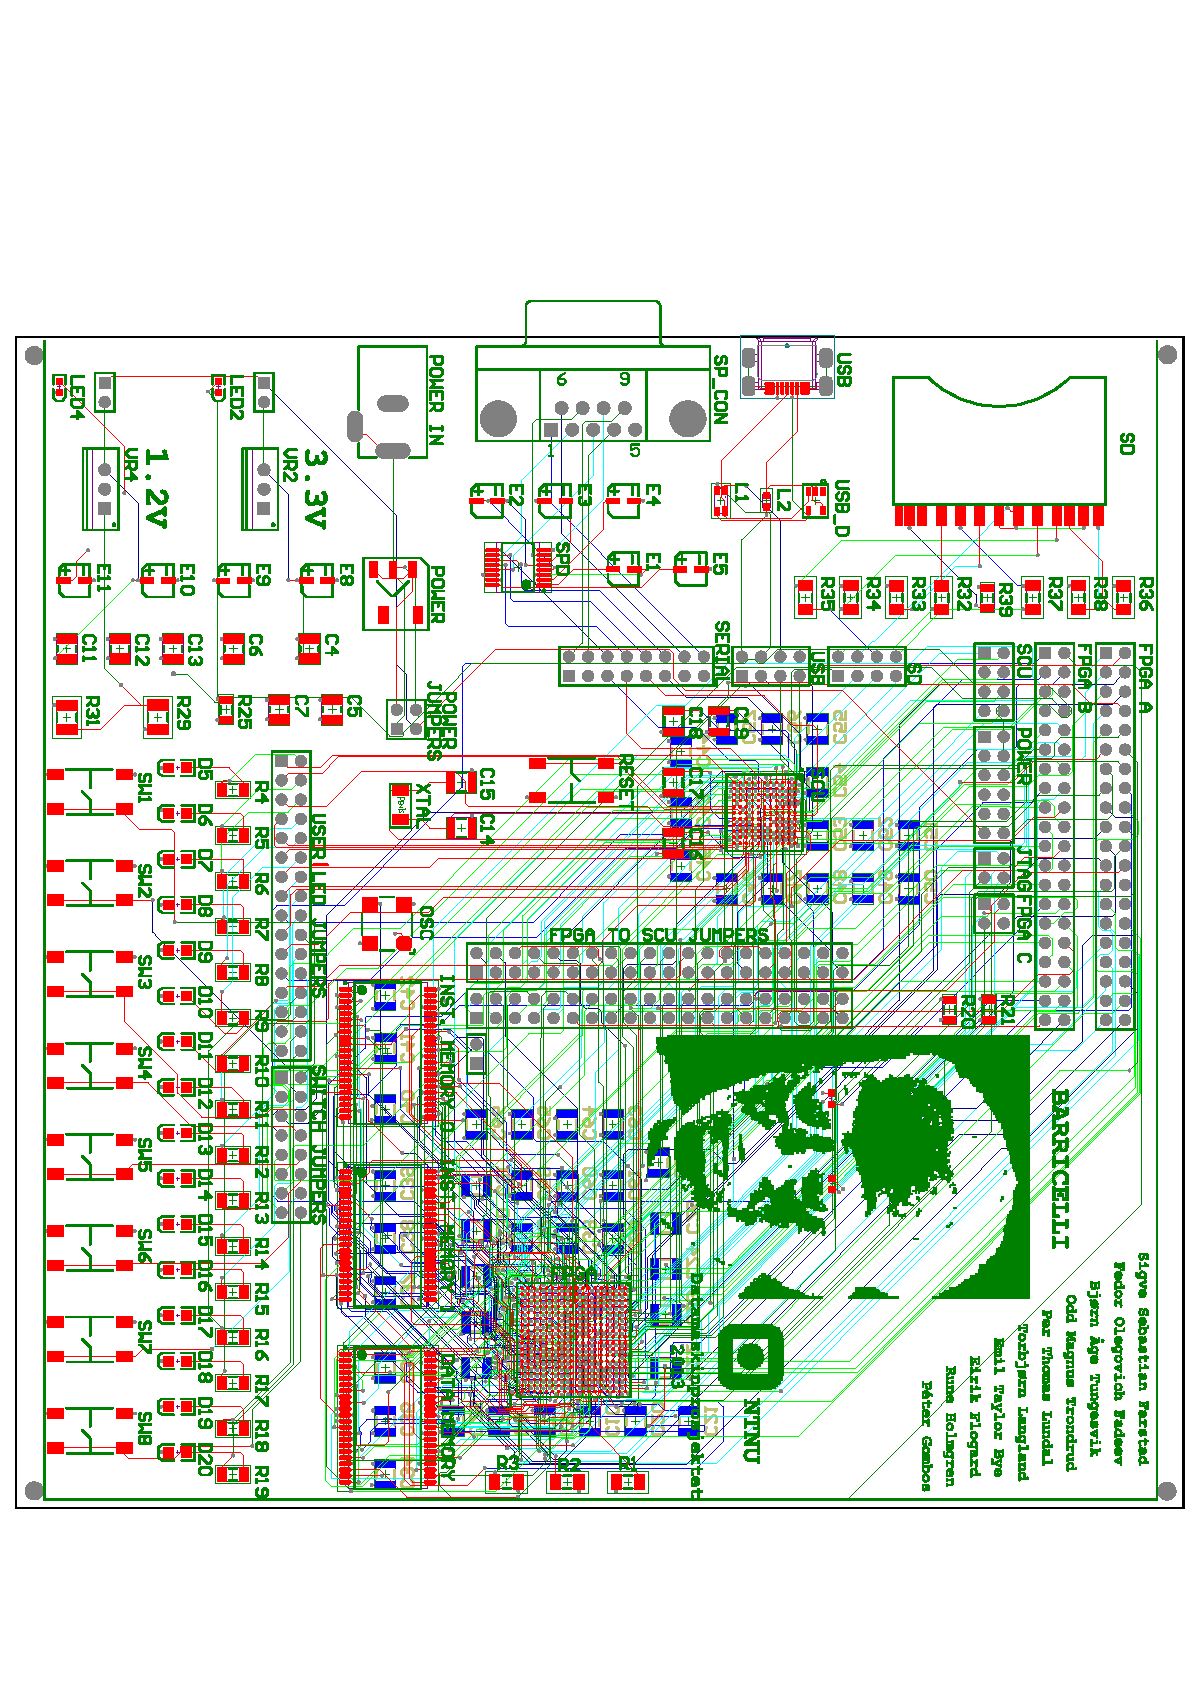
\includepdf[pages=-]{appendix/PCB_TDT4295_NTNU_2013_rotated.18.pdf}

\chapter{Case schematics} \label{appendix:case-schematics}
\newpage

\chapter{Galapos Assembler Listing} \label{appendix:galapagos-assembler-source-code}
\newpage

\lstinputlisting[language=Python]{galapagos-assembler/galapagos/__init__.py}
\lstinputlisting[language=Python]{galapagos-assembler/galapagos/assembler.py}
\lstinputlisting[language=Python]{galapagos-assembler/galapagos/base.py}
\lstinputlisting[language=Python]{galapagos-assembler/galapagos/instructions.py}
\lstinputlisting[language=Python]{galapagos-assembler/galapagos/scanner.py}

\chapter{Demonstration Program Listings} \label{appendix:demonstration-programs-source-code}
\newpage

\lstinputlisting[language={[x86masm]Assembler}]{GAS-programs/knapsack/solver.gas}
\lstinputlisting[language={[x86masm]Assembler}]{GAS-programs/simple_memtest/memtest.gas}

\chapter{Test Bench Documentation} \label{appendix:test-bench-documentation}
\newpage

\section{Introduction}
\todo{ Find a way to convert 0 to G}
This document provides additional documentation and graphics from unit test benches, used for verifyring the components in the FPGA.
The graphics are selected screenshots taken in ISim\cn.  

\section{Component Tests}

\subsection{Fitness Core}
\todo{ MUST...WRITE...SOMETHING?!}

\subsection{Genetic Pipeline}

\subsubsection{Selection Core}
\subsubsection{Crossover Core} 
\begin{figure}[H]
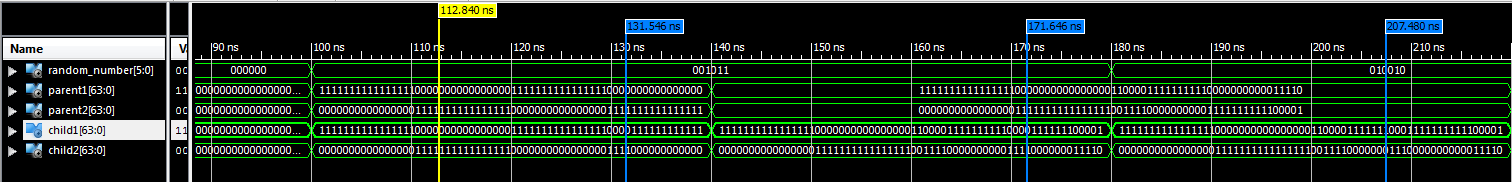
\includegraphics[width=\textwidth]{fpga/fig/testbenches/crossover_split_simulation1.png}
\caption{Crossover Split Simulation Screenshot}
\label{fig_crossover_split_testbench}
\end{figure}

Figure \ref{fig_crossover_split_testbench} shows the simulation of Crossover Split function, where the blue markers are set just before the crossover begins. 
Changes in input parents and random\_number causes changes in children. 

\begin{figure}[H]
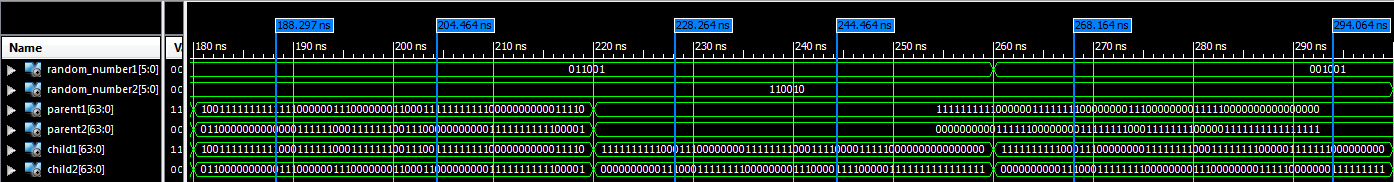
\includegraphics[width=\textwidth]{fpga/fig/testbenches/crossover_doublesplit_simulation1.png}
\caption{Crossover Double-Split Simulation Screenshot}
\label{fig_crossover_doublesplit_testbench}
\end{figure}

Figure \ref{fig_crossover_doublesplit_testbench} shows the simulation of Crossover Double-Split function, where the blue markers are set alternating before and after crossover.
Changes in input parents and any random\_number causes changes in children. 

\begin{figure}[H]
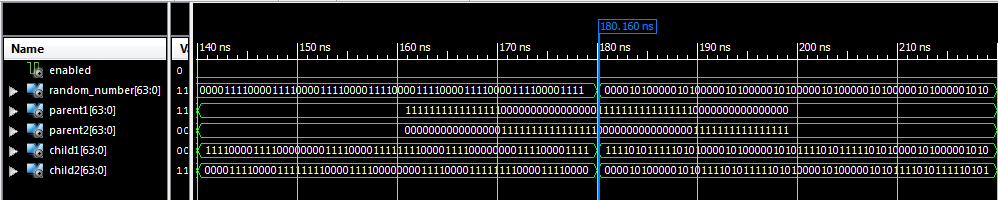
\includegraphics[width=\textwidth]{fpga/fig/testbenches/crossover_xor_simulation1.png}
\caption{Crossover XOR Simulation Screenshot}
\label{fig_crossover_xor_testbench}
\end{figure}

Figure \ref{fig_crossover_xor_testbench} shows the simulation of Crossover XOR function, where the blue marker is set at a change in the random\_number, causing changes on the crossover in the children.
Changes in input parents and any random\_number causes changes in children. 

\begin{figure}[H]
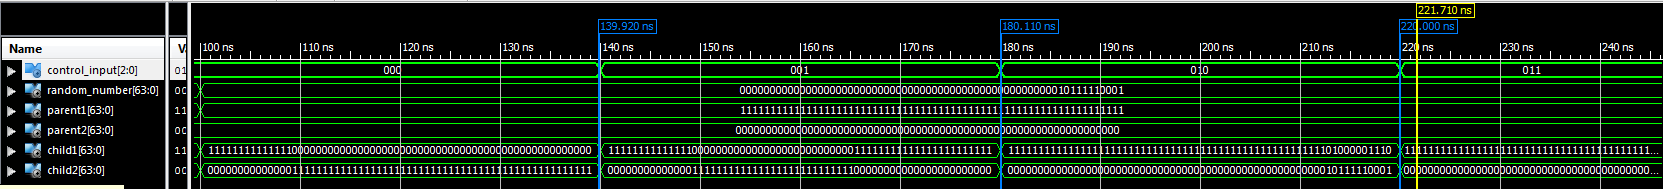
\includegraphics[width=\textwidth]{fpga/fig/testbenches/crossover_toplevel_testbench.png}
\caption{Crossover Toplevel Simulation Screenshot}
\label{fig_crossover_toplevel_testbench}
\end{figure}

Figure \ref{fig_crossover_toplevel_testbench} shows the simulation of Crossover toplevel, where the blue markers are set at changes in the control\_input, changing from split to double-split, then to XOR, and finally to no crossover at all.

\subsubsection{Mutation Core}
\begin{figure}[H]
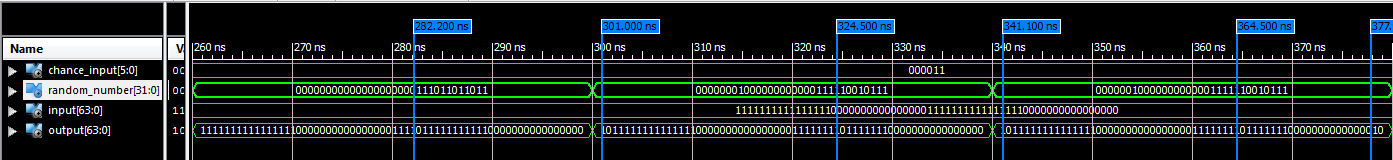
\includegraphics[width=\textwidth]{fpga/fig/testbenches/mutation_simulation1.png}
\caption{Mutation Core Simulation Screenshot 1}
\label{fig_mutation_testbench1}
\end{figure}

Figure \ref{fig_mutation_testbench1} shows the simulation of the Mutation Core, where the blue markers are set just before the bits that are mutated in the output.
Figure \ref{fig_mutation_testbench2} shows another part of the same simulation, with different main input.

\begin{figure}[H]
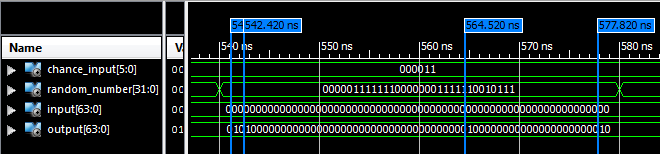
\includegraphics[width=\textwidth]{fpga/fig/testbenches/mutation_simulation2.png}
\caption{Mutation Core Simulation Screenshot 2}
\label{fig_mutation_testbench2}
\end{figure}


\chapter{Budget} \label{appendix:budget}
\newpage
